\chapter{Some formulas and applications}\label{chap8:chap8}

In \pageoriginale this chapter we assume that all the manifolds we
consider are of 
dimension greater than or equal to two.

\section{The second variation formula}\label{chap8:sec1}

To investigate whether a geodesic $\gamma$ with $\gamma(0)=m$,
$\gamma(1)=n$ belongs to $\mathscr{T}(m,n)$ or not, we are led to
proceed as follows (where we use the notations of (\ref{chap2:sec8}) and
(\ref{chap4:sec1}).

\subsection{}\label{chap8:8.1.1}
Let $f$ be a one parameter family
$$
f:]-\epsilon, 1+\epsilon[\times J\to M(\epsilon >0)
$$
with fixed end points, i.e.
$$
f(0,\alpha)=\gamma(0)\quad\text{and}\quad f(1,\alpha)=\gamma(1) \; \forall
\alpha \in J,
$$
and such that $f_{0}=\gamma$. Then the first variation formula (see
\eqref{chap4:4.1.2}, (\ref{chap5:5.2.1})) gives that
$$
l'_{f}(0)=\frac{\partial}{\partial \alpha}(\lg(f_{\alpha}|[0,1])=0.
$$
Then if $\gamma$ is in $\mathscr{T}(\gamma(0),\gamma(1))$, we have
$$
\lg(f_{\alpha}|[0,1])\geq \lg(\gamma|[0,1])=\lg(f_{0}|[0,1]);
$$
therefore the so-called {\em second variation} $l''_{f}(0)$ verifies:
$$
l''_{f}(0)=\frac{\partial^{2}}{\partial
  \alpha^{2}}(\lg(f_{\alpha}|[0,1]))\geq 0.
$$
Later on we will use the fact that $l''_{f}(0)<0$ implies that
$\gamma\not\in \mathscr{T}(m,n)$ (see (\ref{chap8:coro8.1.12}). So we wish to
compute $l''_{f}(0)$.

\subsection{}\label{chap8:8.1.2}\pageoriginale
Now let us assume that $f$ is such that
\begin{itemize}
\item[i)] $f_{0}$ is a geodesic parametrised by the arc length,

\item[ii)] $g(\uub{P},\uub{Q})(t,0)=0$ and then compute $l''_{f}(0)$
  (we do not require that the end points be fixed).
\end{itemize}

We have
\begin{align*}
l''_{f}(0)&=\frac{\partial^{2}}{\partial\alpha^{2}}(\lg(f_{\alpha}|[0,1]))\\
&=\ldots
\ldots=Q(Q\int\limits^{1}_{0}g(\uub{P},\uub{P})^{1/2}\dt))\\
&=\int\limits^{1}_{0}Q(Q(g(\uub{P},\uub{P})^{1/2}))\dt;\tag{8.1.3}\label{chap8:8.1.3}
\end{align*}
\begin{align*}
Q(g(\uub{P},\uub{P})^{1/2})&=1/2\,
Q(g(\uub{P},\uub{P}))g(\uub{P},\uub{P})^{-\frac{1}{2}}\\
&=g(D_{Q}\uub{P},\uub{P})g(\uub{P},\uub{P})^{-\frac{1}{2}}\text{
  \ by (\ref{chap5:5.4.8}) (C.D.7).}\tag{8.1.4}\label{chap8:8.1.4}
\end{align*}
Hence, using the fact that
$$
Q(Q(g(\uub{P},\uub{P})^{1/2}))=Q(g(D_{Q}\uub{P},\uub{P}))g(\uub{P},\uub{P})^{1/2}, 
$$
we obtain
\begin{gather*}
-(1/2)g(D_{Q}\uub{P},\uub{P})\cdot Q(g(\uub{P},\uub{P}))\cdot
g(\uub{P},\uub{P})^{-3/2}=\ldots\tag{8.1.5}\label{chap8:8.1.5}\\
\ldots=g(D_{Q}D_{Q}\uub{P},\uub{P})+g(D_{Q}\uub{P},D_{Q}\uub{P})g(\uub{P},\uub{P})^{\frac{1}{2}}-g(D_{Q}\uub{P},\uub{P})^{2}g(\uub{P},\uub{P})^{-3/2}. 
\end{gather*}
Now we use (\ref{chap8:8.1.2}). We have
\begin{align*}
g(D_{Q}\uub{P},\uub{P}) &= g(D_{P}\uub{Q},\uub{P})\text{ since }
[\uub{P},\uub{Q}]=0\text{ and } D \text{ is symmetric}\\
&= P(g(\uub{Q},\uub{P}))-g(\uub{Q},D_{P},\uub{P})\text{ by (\ref{chap5:5.4.8}).} 
\end{align*}
Since $f_{0}$ is a geodesic $(D_{P}\uub{P})(t,0)=0$ and hence by
(\ref{chap8:8.1.2}) ii) we have
\begin{equation*}
g(D_{Q}\uub{P},\uub{P})(t,0)=0.\tag{8.1.6}\label{chap8:8.1.6} 
\end{equation*}
Again \pageoriginale since $D$ is symmetric and $[\uub{P},\uub{Q}]=0$
we have
\begin{align*}
g(D_{Q}D_{Q}\uub{P},\uub{P}) &=
g(D_{Q}D_{P}\uub{Q},\uub{P})=g(D_{P}D_{Q}\uub{Q},\uub{P})+g(R(\uub{Q},\uub{P})\uub{Q},\uub{P})\\
&\hspace{4cm} \text{ by (\ref{chap2:2.5.12}) (C.D.5)}\\
&=
P(g(D_{Q}\uub{Q},\uub{P}))-g(D_{Q}\uub{Q},D_{P}\uub{P})+g(R(\uub{P},\uub{Q})\uub{P},\uub{Q}). 
\end{align*}
Now since $f_{0}$ is a geodesic we have $(D_{P}\uub{P})(t,0)=0$ and
hence we have
\begin{equation*}
g(D_{Q}D_{Q}\uub{P},\uub{P})(t,0)=P(g(D_{Q}\uub{Q},\uub{P}))(t,0)+g(R(\uub{P},\uub{Q})\uub{P},\uub{Q})(t,0).\tag{8.1.7}\label{chap8:8.1.7} 
\end{equation*}
Combining \eqref{chap8:8.1.5}, \eqref{chap8:8.1.6} and \eqref{chap8:8.1.7} with the fact
that $f_{0}$ is parametri\-sed by the arc length and hence
$g(\uub{P},\uub{P})(t,0)=1$ we have the following proposition.

\setcounter{prop}{7}
\begin{prop}\label{chap8:prop8.1.8}
If $f$ is a one parameter family of curves satisfying the conditions
(\ref{chap8:8.1.2}) {\rm (i)} and {\rm (ii)} then
$$
l''_{f}(0)=\left[g(D_{Q}\uub{Q},\uub{P})\right]^{(1,0)}_{(0,0)}+\int\limits^{1}_{0}(||D_{P}\uub{Q}||^{2}+g(R(\uub{P},\uub{Q})\uub{P},\uub{Q}))(t,0)\dt 
$$
Noticing the fact that the integral in (\ref{chap8:prop8.1.8}) depends only
on the curve $f_{0}$ and on the lift $Q(t,0)$ of that curve we give
the following definition.
\end{prop}

\setcounter{definition}{8}
\begin{definition}\label{chap8:defi8.1.9}
Let
$$
\gamma:[0,1]\to M
$$
be a curve and let $h$ be a lift of $\gamma$ into $T(M)$.

Then we define
$$
l''_{h}(0)=\int\limits^{1}_{0}(||D_{P}h||^{2}+g(R(\gamma',h)\gamma',h))(t)\dt. 
$$
In \pageoriginale general it is easier to construct a lift $h$ along a
curve $\gamma$ and compute $l''_{h}(0)$ then to construct a family $f$
of curves and compute $l''_{f}(0)$. A relation between the two
processes is given by the:
\end{definition}

\setcounter{prop}{9}
\begin{prop}\label{chap8:prop8.1.10}
Let
$$
\gamma:[0,1]\subset I\to (M,g)
$$
be a geodesic parametrised by the arc length and let $h$ be a lift of
$\gamma$ into $T(M)$ such that
$$
g(\gamma',h)=0.
$$
Then, there exists an interval $J$ containing zero and a one parameter
family
$$
f:]-\epsilon, 1+\epsilon[\times J\to M(\epsilon>0)
$$
of curves such that
\begin{itemize}
\item[\rm a)] $f_{0}=\gamma$ and (\ref{chap8:8.1.2}) {\rm i) ii)} hold for
  $f$

\item[\rm b)] $l''_{f}(0)=l''_{h}(0)$.
\end{itemize}
\end{prop}

\begin{proof}
We wish to set:
$$
f(t,\alpha)=\exp(\alpha\cdot h(t)).
$$
But the right hand side makes sense only if $\alpha\cdot h(t)\in
\Omega$. So we adjust $J$ so that this happens. Let
$0<\epsilon'<\epsilon$; the map
$$
[-\epsilon',1+\epsilon']\times J\ni (t,\alpha)\to \alpha\cdot h(t)\in T(M)
$$
is continuous. Under this map the compact set $[-\epsilon',
  1+\epsilon']\times\{0\}$ goes into the open set $\Omega$ since
$\Omega\ni 0_{P}\forall p\in M$. Hence there exists $r>0$ such that
under the above map $[-\epsilon',1+\epsilon']\times[-r,r]$ goes into
$\Omega$. Hence we can set
$$
f(t,\alpha)=\exp(\alpha\cdot h(t))\forall
(t,\alpha)\epsilon[-\epsilon',1+\epsilon']\times[-r,r]. 
$$
Then\pageoriginale
$$
f_{0}(t)=\exp(0\cdot
h(t))=\exp(0_{p(h(t))})=\exp(0_{\gamma(t)})=\gamma(t)
$$
and hence $f_{0}$ is a geodesic parametrised by the arc length; and
since $\uub{Q}(t,0)=h(t)$ we have
$$
g(\uub{P},\uub{Q})(t,0)=g(\gamma',h)(t)=0.
$$
\end{proof}

\setcounter{subsection}{10}
\subsection{}\label{chap8:8.1.11}
Hence $f$ satisfies a) i). For ii) we see that $h(t)=\uub{Q}(0,t)$ (as
in (\ref{chap2:sec8})), and hence:
$$
l''_{f}(0)=\left[g(D_{Q}\uub{Q},\uub{P})\right]^{(1,0)}_{(0,0)}+\int\limits^{1}_{0}(||D_{P}\uub{Q}||^{2}+g(R(\uub{P}\uub{Q})\uub{P},\uub{Q}))(t,0)\dt. 
$$
But since the map
$$
\alpha\to \exp(\alpha\cdot h(t))
$$
is a geodesic we have
$$
(D_{Q}\uub{Q})=0.
$$
Hence we are through by (\ref{chap8:8.1.11}) and the definition of
$l''_{h}(0)$. 

\setcounter{coro}{11}
\begin{coro}\label{chap8:coro8.1.12}
Let $m$ and $n$ be points of $M$ and let $\gamma\in\mathscr{P}(m,n)$
be a geodesic in $(M,g)$; suppose that there exists a lift $h(t)$ of
$\gamma$ such that
\begin{itemize}
\item[\rm 1)] $g(h,\gamma')=0$,

\item[\rm 2)] $h(0)=h(1)=0$,

\item[\rm 3)] $l''_{h}(0)<0$.
\end{itemize}
Then $\gamma\not\in \mathscr{T}(m,n)$.
\end{coro}

\begin{proof}
Let us take the one parameter family defined in the above
proposition. Then we have
$$
\frac{\partial}{\partial\alpha}(\lg(f_{\alpha}|[0,1]))=0
$$
and\pageoriginale
$$
\frac{\partial^{2}}{\partial
  \alpha^{2}}(\lg(f_{\alpha}|[0,1]))=l''_{r}(0)=l''_{h}(0)<0.
$$
Hence using Taylor's formula with a remainder we see that there exist
$\alpha$'s such that
\begin{equation*}
g(f_{\alpha}|[0,1])<g(f_{0}|[0,1]).\tag{8.1.13}\label{chap8:8.1.13}
\end{equation*}
But we have
\begin{align*}
f(0,\alpha) &= \exp(\alpha\cdot h(0))=\exp(\alpha\cdot
0_{\gamma(0)})=\gamma(0)=m\\
\text{and}\qquad f(1,\alpha) &= \exp(\alpha\cdot
h(1))=\exp(\alpha\cdot 0_{\gamma(1)})=\gamma(1)=n
\end{align*}
and hence by \eqref{chap8:8.1.13} there exist curves from $m$ to $n$ with
length less than that of $\gamma$. Hence $\gamma$ is not in
$\mathscr{T}(m,n)$. 
\end{proof}

\section{Second variation versus Jacobi fields}\label{chap8:sec2}

\subsection{}\label{chap8:8.2.1}

\begin{notation*}
For $x\in U(M)$ let us set (see (\ref{chap2:2.8.30})):
$$
j(x)=\inf\{t>0|\gamma_{x}(0)\text{ \  and \ }\gamma_{x}(t)\text{ \ are
  conjugate on \ } \gamma_{x}\}.
$$
If $\exp_{m}$ is $r$-O.K.\@ then by (\ref{chap2:2.8.32}) it follows that
$$
j(x)\geq r \; \forall x\in U_{m}(M).
$$
Hence $j(x)$ is a strictly positive function on $U(M)$.
\end{notation*}


\subsection{}\label{chap8:8.2.2}

\begin{prop*}
Let $x\in U(M)$, $l\in [0,j(x)]$ and let
$$
h:[0,1]\to T(M)
$$
be a lift of $\gamma_{x}$ such that $h(0)=h(1)=0$. Then
$l''_{h}(0)\geq 0$ and equality holds if and only if $h$ is a Jacobi field.
\end{prop*}

\begin{proof}
Let $\{x=x_{1},x_{2},\ldots,x_{d}\}$ be a basis of $T_{m=p(x)}(M)$ and
let $h_{i}$ be the Jacobi field along $\gamma_{x}$ such that
$h_{i}(0)=0$ and $(D_{P}h_{i})(0)=x_{i}$ (see
(\ref{chap2:2.8.26})). {\em Then $\forall t\in
  [0,1]:\{h_{1}(t),\ldots,h_{d}(t)\}$ form a basis of}
$T_{\gamma_{x}(t)}(M)$: for if for some $t_{0}>0$ we have:
$$
\sum_{i}a_{i}h_{i}(t_{0})=0.
$$
then \pageoriginale the Jacobi field $k:t\to \sum\limits_{i}a_{i}h(t)$
vanishes at $t=0$ and at $t=t_{0}$ so by (\ref{chap2:2.8.30}): $k=0$.

Hence
$$
D_{P}k=\sum_{i}a_{i}D_{P}h_{i}=0;
$$
in particular
$$
(D_{P}k)(0)=\sum\limits_{i}a_{i}x_{i}=0.
$$
Since $\{x_{1},\ldots,x_{d}\}$ is a basis of $T_{m}(M)$ we have
$$
a_{1}=\ldots=a_{d}=0.\qquad\text{Q.E.D.}
$$
Hence corresponding to every lift $h$ of $\gamma_{x}$ into $T(M)$ we
have functions $\{f_{1},\ldots,f_{d}\}$ on $]0$, $1[$ such that
\begin{equation*}
h(t)=\sum_{i}f_{i}(t)h_{i}(t).\tag{8.2.3}\label{chap8:8.2.3}
\end{equation*}
Then we have
$$
D_{P}h=\sum_{i}f'_{i}h_{i}+\sum_{i}f_{i}(D_{P}h_{i})
$$
and setting
\begin{equation*} 
u=\sum_{i}f'_{i}h_{i}\quad\text{and}\quad
v=\sum_{i}f_{i}(D_{P}h_{i})\tag{8.2.4}\label{chap8:8.2.4} 
\end{equation*}
we have
$$
D_{P}h=u+v.
$$
Hence
\begin{equation*}
||D_{P}h||^{2}=||u||^{2}+2g(u,v)+||v||^{2}\tag{8.2.5}\label{chap8:8.2.5}
\end{equation*}
and
\begin{align*}
g(R(\gamma'_{x},h)\gamma'_{x},h) &= g(R(\gamma'_{x},\sum
f_{i}h_{i})\gamma'_{x},h)=\tag{8.2.6}\label{chap8:8.2.6}\\
&=\sum_{i}f_{i}g(R(\gamma'_{x},h_{i})\gamma'_{x},h)=\sum_{i}f_{i}g(D_{P}D_{P}h_{i},h),\\
&\quad \text{(since $h_{i}$ are Jacobi fields).}
\end{align*}
\end{proof}

\setcounter{subsection}{5}
\subsection{}\label{chap8:8.2.6a}\pageoriginale
\begin{align*}
& =g(\sum_{i}f_{i}D_{P}D_{P}h_{i},h)=g(D_{P}v-\sum_{i}f'_{i}D_{P}h_{i},h)\\
&=g(D_{P}v,h)-\sum_{i}f'_{i}g(D_{P}h_{i},h).\\
&=P(g(v,h))-g(v,D_{P}h)-\sum_{i,j}f'_{i}f_{j}g(D_{P}h_{i},h_{j}=\\
&\hspace{5cm} \text{ by (\ref{chap5:5.4.8}) (C.D.7)}\\
& =P(g(v,h))-g(v,u+v)-\sum_{i,j}f'_{i}f_{j}g(D_{P}h_{i},h_{j}).
\end{align*}
But if we set
$$
\xi=g(D_{P}h_{i},h_{j})-g(D_{P}h_{j},h_{i})\quad\text{(a classical
  Sturmain argument)}
$$
then 
\begin{align*}
\xi'=P(\xi) &=
g(D_{P}D_{P}h_{i},h_{j})+g(D_{P}h_{i},D_{P}h_{j})\\
&\qquad-g(D_{P}D_{P}h_{j},h_{i})-g(D_{P}h_{j},D_{P}h_{i})\\
&= g(D_{P}D_{P}h_{i},h_{j})-g(D_{P}D_{P}h_{j},h_{i})=\\
&=
g(R(\gamma'_{x},h_{i})\gamma'_{x},h_{j})-g(R(\gamma'_{x},h_{j})\gamma'_{x},h_{i})=0\\
&\hspace{6cm} \text{ by \eqref{chap5:5.5.5C.T.4}.}
\end{align*}
Hence $\xi$ is constant, but $\xi(0)=0$ for $h_{i}(0)=0\forall i$. So
$\xi=0$. Hence we have
\begin{align*}
\sum_{i,j}f'_{i}f_{j}g(D_{P}h_{i},h_{j})&=\sum_{i,j}f'_{i}f_{j}g(D_{P}h_{j},h_{i})\\
&=g(\sum_{j}f_{j}D_{P}h_{j},\sum_{i}f'_{i}h_{i})=g(u,v). 
\end{align*}
Hence by \eqref{chap8:8.2.5} and \eqref{chap8:8.2.6} we have
$$
||D_{P}h||^{2}+g(R(\gamma'_{x},h)\gamma'_{x},h)=P(g(v,h))+||u||^{2}.
$$
Hence\pageoriginale
$$
l''_{h}(0)=\left[g(v,h)\right]^{1}_{0}+\int\limits^{1}_{0}||u||^{2}\dt,
$$
and since $h(0)=h(1)=0$ we have
\begin{equation*}
l''_{h}(0)=\int\limits^{1}_{0}||u||^{2}\dt.\tag{8.2.7}\label{chap8:8.2.7}
\end{equation*}
Hence $l''_{h}(0)\geq 0$ and equality holds if and only if $u$ is
identically zero. But since $\{h_{1}(t),\ldots,h_{d}(t)\}$ from a
basis for every $t$, $u$ is identically zero if and only if each
$f'_{i}$ is zero, i.e.\@ if and only if each $f_{i}$ is a constant.

Hence $h=\sum\limits_{i}f_{i}h_{i}$ is a Jacobi field.

\setcounter{subsection}{8}\label{chap8:8.2.9}
\subsection{}


\begin{prop*}
Let $x\in U(M)$ and $l>j(x)$; then 
$$
\gamma_{x}|[0,1]\in \mathscr{T}(\gamma_{x}(0), \gamma_{x}(1)).
$$
\end{prop*}

\begin{proof}
First we prove two lemmas.
\end{proof}

\setcounter{subsection}{9}

\subsection{}\label{chap8:8.2.10}

\begin{lemma*}
Let $h$ be a Jacobi field along $\gamma_{x}$. Then
$$
l''_{h}(0)=\left[g(D_{p}h,h)\right]^{1}_{0}.
$$
\end{lemma*}

\begin{proof}
We have by definition
\begin{align*}
l''_{h}(0) &=
\int\limits^{1}_{0}g(D_{p}h,D_{P}h)+g(R(\gamma'_{x},h)\gamma'_{x},h)\dt=\\
&= \int\limits^{1}_{0}g(D_{P}h,D_{P}h)+g(D_{P}D_{P}h,h)\dt\text{
  \ (since $h$ is a Jacobi field)}\\
&= \int\limits^{1}_{0}P(g(D_{P}h,h))\dt\text{ \ by (\ref{chap5:5.4.8}) (C.D.7)}
=\left[g(D_{P}h,h)\right]^{1}_{0}. 
\end{align*}
\end{proof}

\subsection{}\label{chap8:8.2.11}

\begin{lemma*}
Let $h$ be a Jacobi field along $\gamma_{x}$ such that
$$
h(0)=0\quad\text{and}\quad (D_{P}h)(0)\neq 0.
$$
Then given any positive number $\eta$ we can choose a positive number
$\epsilon$ less\pageoriginale than $\eta$ and a Jacobi field $k$ along
$\gamma_{x}|[-\epsilon,\epsilon]$ such that
\begin{itemize}
\item[\rm i)] $k(-\epsilon)=h(-\epsilon)$

\item[\rm ii)] $k(\epsilon)=0$

\item[\rm iii)] $g(D_{P}h,h)(-\epsilon)<g(D_{P}k,k)(-\epsilon)$.
\end{itemize}
\end{lemma*}

\begin{proof}
Let $r$ be a positive number such that $B(m,r)$ is convex. Then
$\forall t\in ]0$, $r[$ there exists a Jacobi field $k_{t}$ along
    $\gamma|[-t,t]$ such that
\begin{equation*}
k_{t}(-t)=h(t)\quad\text{and}\quad k_{t}(t)=0.\tag{8.2.12}\label{chap8:8.2.12}
\end{equation*}
\begin{figure}[H]
\centering
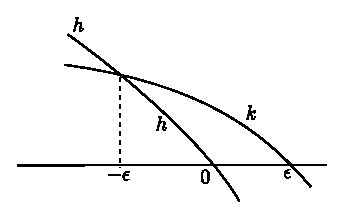
\includegraphics{figures/chap8-fig1.eps}
\end{figure}

In fact we set $f_{\alpha}=$ the geodesic from $\exp(\alpha\cdot
h(-t))$ to $\gamma(t)$ parametri\-sed by the arc length, then the family
$\{f_{\alpha}\}$ of the curves $f_{\alpha}$ so obtained is a
one-parameter family of geodesics and the $k(s)=\uub{Q}(s,0)$ satisfy
our requirements. Now let us set
$$
u=(D_{P}h)(0)\quad\text{and}\quad \widehat{k}_{t}(t')=a_{t}+t'b_{t}+0(t').
$$
Then
$$
\widehat{h}(t')=t'\cdot u+0(t'),\widehat{h}'(t')=u+0(1)
$$
and 
$$
\widehat{k}'_{t}(t')=b_{t}+0(1).
$$
Then by \eqref{chap8:8.2.12} we have
$$
a_{t}-tb_{t}+0(t)=\widehat{k}_{t}(-t)=\widehat{h}(-t)=-tu+0(t)
$$
and
$$
\widehat{k}_{t}(t)=a_{t}+tb_{t}+0(t)=0.
$$
Hence\pageoriginale
$$
b_{t}=\frac{u}{2}+0(t).
$$
\end{proof}
 
\setcounter{subsection}{12}
\subsection{}\label{chap8:8.2.13}
Hence
$$
g(D_{P}h,h)(-t)=g(\widehat{h}'(-t),\widehat{h}(-t))=g(u+0(1),-tu+0(t))=-t||u||^{2}+0(t), 
$$
and
\begin{gather*}
g(D_{P}k_{t},k_{t})(-t)=g(\widehat{k}'_{t}(-t),\widehat{k}_{t}(-t))\\
=g\left(\frac{u}{2}+0(1),
\widehat{h}(-t)\right)=g\left(\frac{u}{2}+0(1),
-tu+0(t)\right)=\frac{t}{2}||u||^{2}+0(t). 
\end{gather*}
Since $u$ is non zero by our hypothesis we have $||u||>0$ and hence by
(\ref{chap8:8.2.13}) we can choose $t$ so small that
$$
g(D_{P}h,h)(-t')<g(D_{P}k,k)(-t')
$$
for $0<t'<t$.

Now let us take up the proof of (\ref{chap8:8.2.9}). Since $1>j(x)$
there exists a $t_{0}\in ]0$, $1[$ and a Jacobi field $h$ along
    $\gamma_{x}$ such that
$$
h\neq 0, h(0)=h(1)=0.
$$
Set $\eta=-t_{0}$. Then applying the lemma (\ref{chap8:8.2.11}) for the
Jacobi field $h$ around the point $t_{0}$ we get $\epsilon \in ]0$,
  $\eta[$ and a Jacobi field $k_{\epsilon}$ along
    $\gamma_{x}|[t_{0}-\epsilon, t_{0}+\epsilon]$. Now let $f$ be the
    lift of $\gamma_{x}$ such that:
\begin{align*}
h_{1} &= f|[0,t_{0}-\epsilon]=h|[0,t_{0}-\epsilon]\\
h_{2} &= f|[t_{0}-\epsilon, t_{0}+\epsilon]=k_{\epsilon}\\
h_{3} &= f|[t_{0}+\epsilon,1]=0.
\end{align*}
Then \pageoriginale we have
$$
l''_{f}(0)=l''_{h_{1}}(0)+l''_{h_{2}}(0)+l''_{h_{3}}(0).
$$
But by (\ref{chap8:8.2.10}) we have
$$
l''_{h_{1}}(0)=\left[g(D_{P}h_{1},h_{1})\right]^{1-\epsilon}_{0}=g(D_{P}h_{1},h_{1})(1-\epsilon)\text{
  \  since \ } h_{1}(0)=h(0)=0;
$$
and 
$$
l''_{h_{2}}(0)=\left[g(D_{P}h_{2},h_{2})\right]^{1+\epsilon}_{1-\epsilon}=-g(D_{P}h_{2},h_{2})(1-\epsilon)\text{
  \ since \ } h_{2}(1+\epsilon)=0
$$
and 
$$
l''_{h_{3}}(0)=0\text{ \  since \ } h_{3}=0.
$$
Hence $l''_{f}(0)<0$ so we are done with (\ref{chap8:coro8.1.12}).

\setcounter{subsection}{13}

\subsection{}\label{chap8:8.2.14}

\begin{remark*}
The two propositions (\ref{chap8:8.2.2}) and (\ref{chap8:8.2.9}) are
essential parts of Morse's index theorem.
\end{remark*}

\section{The theorems of Synge and Myers}\label{chap8:sec3}

First let us recall that Ricci curvature $(\Ric)$ is a function from
$T(M)$ to $\mathbb{R}$.

\subsection{}\label{chap8:8.3.1}

\begin{prop*}
Let $(M,g)$ be an r.m.\@ of dimension $d$ such that
$$
\Ric(U(M))\subset [k,\infty[
$$ 
for some $k>0$. Let $\gamma$ be a geodesic in $\mathscr{P}(m,n)$ where
$m$ and $n$ are points of $M$. Now if
$$
\lg(\gamma)>\pi\left(\frac{d-1}{k}\right)^{1/2}
$$
then \pageoriginale $\gamma\not\in \mathscr{T}(m,n)$.
\end{prop*}

\begin{proof}
Let us suppose that $\gamma$ is parametrised by the arc length and
then take an orthonormal basis
$\{x_{1}=\gamma'(0),x_{2},\ldots,x_{d}\}$ of $T_{\gamma(0)}(M)$. Let
$h_{i}$ be the parallel lift along $\gamma$ with $h_{i}(0)=x_{i}$, and
set
$$
s_{i}(t)=\sin\left(\frac{\pi}{1}t\right)\cdot h_{i}(t).
$$
Then since $h_{i}$ is a parallel lift we have $D_{P}h_{i}=0$ and hence
by (\ref{chap2:2.4.1}) D.L.3 we have
$$
(D_{P}s_{i})(t)=\frac{\pi}{1}\cos\left(\frac{\pi t}{1}\right)\cdot
h_{i}(t), 
$$
and since parallel transport preserves $g$ we have
\begin{equation*}
||(D_{P}s_{i})(t)||^{2}=\frac{\pi^{2}}{1^{2}}\cos^{2}\left(\frac{\pi
  t}{1}\right).\tag{8.3.2}\label{chap8:8.3.2} 
\end{equation*}
Again since parallel transport preserves $g$ by the definition of $A$
(see \eqref{chap6:6.1.2}) and since $\gamma'(0)$ and $h_{i}(0)$ are
orthogonal we have
$$
g(R(\gamma',h)\gamma',h)=-A(\gamma',s_{i})||s_{i}||^{2}=-A(\gamma',h_{i})\sin^{2}\frac{\pi
  t}{1}. 
$$
Hence by the definition (\ref{chap8:defi8.1.9}) we have
\begin{equation*}
l''_{s_{i}}(0)=\int\limits^{1}_{0}\frac{\pi^{2}}{1^{2}}\cos^{2}\left(\frac{\pi}{1}t\right)-\sin^{2}\left(\frac{\pi
  t}{1}\right)A(\gamma',h_{i})\dt.\tag{8.3.3}\label{chap8:8.3.3}
\end{equation*}
By (\ref{chap6:6.8.6}) we have
$$
\sum^{d}_{i=2}A(\gamma',h_{i})=\Ric(\gamma')\geq k
$$
and hence
\begin{equation*}
\sum^{d}_{i=2}l''_{s_{i}}(0)\leq
\int\limits_{0}\frac{\pi^{2}}{l^{2}}\cdot (d-1)\cos^{2}\left(\frac{\pi
  t}{1}\right)-k\sin^{2}\left(\frac{\pi t}{1}\right)\dt=\frac{1}{2}\left(\frac{\pi^{2}}{1^{2}}(d-1)-k\right).\tag{8.3.4}\label{chap8:8.3.4}
\end{equation*}
Hence \pageoriginale if
$l>\pi\left(\dfrac{d-1}{k}\right)^{\frac{1}{2}}$ then
$\sum\limits^{d}_{i=2}l''_{s_{i}}(0)<0$ and hence
$$
\exists\, i|l''_{s_{i}}(0)<0;
$$
hence, by (\ref{chap8:coro8.1.12}), $\gamma\not\in \mathscr{T}(m,n)$.
\end{proof}

\setcounter{subsection}{4}

\subsection{}\label{chap8:8.3.5}

\begin{defi*}
The real number $d(M,g)$ defined as
$$
d(M,g)=\sup \{d(m,n)|m,n\in M\}
$$
is called the {\em diameter of the } r.m.\@ $(M,g)$.
\end{defi*}

\subsection{}\label{chap8:8.3.6}


\begin{remarks*}
\begin{enumerate}
\renewcommand{\labelenumi}{\theenumi)}
\item If $d(M,g)<\infty$ and the manifold $(M,g)$ is complete then by
  Hopf-Rinow theorem it follows that $M$ is compact.

\item Let us note that (\ref{chap6:6.8.6}) implies that if 
$$
A(M)\subset [k,\infty[\text{ then } \Ric(U(M))\subset [(d-1)k,\infty[
$$
\end{enumerate}
\end{remarks*}

\subsection{}\label{chap8:8.3.7}

\begin{coro*}[Myers]
Suppose that $(M,g)$ is a complete r.m.\@ such that there exists a
$k>0$ satisfying
$$
\Ric(U(M))\subset [k,\infty[.
$$
Then
$$
d(M,g)\leq \pi\left(\frac{d-1}{k}\right)^{\frac{1}{2}}.
$$
In particular $M$ is compact and the fundamental group of $M$ is
finite. 
\end{coro*}

\begin{proof}
Suppose that there exist $m$ and $n$ in $M$ such that
$$
d(m,n)>\pi\left(\frac{d-1}{k}\right)^{\frac{1}{2}}.
$$
Then by \eqref{chap8:8.4.8} there exists a geodesic $\gamma$ joining $m$ and
$n$ such that
$$
\lg(\gamma)>\pi\left(\frac{d-1}{k}\right)^{\frac{1}{2}}.
$$
But \pageoriginale this contradicts (\ref{chap8:8.3.1}); hence
$d(M,g)\leq \pi\left(\dfrac{d-1}{k}\right)^{\frac{1}{2}}$.

By (\ref{chap8:8.3.6}) it follows that $M$ is compact. Now let
$$
p:(\widetilde{M},\widetilde{g})\to (M,g)
$$
be the universal riemannian covering of $(M,g)$. Then since $p$ is a
local isometry we obtain
$$
\Ric(U(\widetilde{M}))=\Ric(U(M))\subset [k,\infty[.
$$
Hence the first part of the corollary gives that $\widetilde{M}$ is
compact. Hence the covering $p:\widetilde{M}\to M$ has finite number
of sheets.
\end{proof}

\subsection{}\label{chap8:8.3.8}

\begin{remarks*}
\begin{enumerate}
\renewcommand{\labelenumi}{\theenumi)}
\item This result was first proved by Bonnet for two dimensional
  manifolds.

\item In the above inequality (\ref{chap8:8.3.7}) the equality occurs
  for
$$
\left(\mathbb{S}^{d},\left(\frac{d-1}{k}\right)^{\frac{1}{2}}\cdot
\can\right)\subset 
\mathbb{R}^{d+1}. 
$$
The proof here would not yield easily the result that equality in
(\ref{chap8:8.3.7}) is attained only if $(M,g)$ is isometric to
$(\mathbb{S}^{d}, (\dfrac{d-1}{k})^{\frac{1}{2}}\cdot \can)$. However
the validity of this result can be deduced easily from \cite{33}:
Corollary 4, p.256-257.
\end{enumerate}
\end{remarks*}

\subsection{}\label{chap8:8.3.9}

\begin{theorem*}(Synge)
Let $(M,g)$ be an r.m.\@ such that 
\begin{itemize}
\item[\rm i)] $M$ is compact

\item[\rm ii)] $M$ is orientable

\item[\rm iii)] the dimension of $M$ is even

\item[\rm iv)] $A(M)\subset ]0$, $\infty [$.
\end{itemize}
Then $M$ is simply connected.
\end{theorem*}

\begin{proof}
By \pageoriginale contradiction: suppose that $M$ is not simply
connected; then (see (\ref{chap7:7.6.3})) there exists in $M$ at least one
non-zero free homotopy class. Let $\gamma$ denote the closed geodesic
which fulfills the conditions i) and ii) of theorem
(\ref{chap7:7.6.10}). Let $l=\lg(\gamma)$ and $\tau(t)$ denote the
parallel transport along $\gamma$ from $0$ to $t$. Since
$\gamma(0)=\gamma(1)$ then $\tau(1)$ is an endomorphism of
$T_{\gamma(0)}(M)$; by (\ref{chap5:5.4.9}) we see that $\tau(1)$ belongs
to the orthogonal group of $T_{\gamma{0}}(M)$. In fact $\tau(1)$ is a
rotation. For: suppose that $\sigma$ is the orienting form and that
$\{\gamma'(0)=x_{1},\ldots,x_{d}\}$ is a positive orthonormal base of
$T_{\gamma(0)}(M)$. Then the function
$$
\sigma(\tau(t)(x_{1}),\ldots\ldots,\tau(t)(x_{d}))
$$
never vanishes since $\sigma$ is never zero and $\tau(t)$ is an
isomorphism; hence
$$
\sigma(\tau(1)(x_{1}),\ldots,\tau(1)(x_{d}))=1.
$$
Set
$$
H=\left\{y\in T_{\gamma(0)}(M)|g(\gamma'(0),y)=0\right\};
$$
then since parallel transport preserves $g$ and
$\tau(1)(\gamma'(0))=\gamma'(1)=\gamma'(0)$ by (\ref{chap2:2.3.5}) we get
$\tau(1)(H)=H$. But $H$ is odd dimensional and hence $\exists\, y\in
H$, $y\neq 0$, with $\tau(1)(y)=y$ (because $\tau(1)$ is a rotation).

Let $h$ be the parallel lift of $\gamma$ such that $h(0)=y$. since
$\tau(1)(y)=y$ we have
$$
h(0)=h(1)=y.
$$
Now \pageoriginale let $f$ be the parameter family of curves associated
to $h$ in the manner of (\ref{chap8:prop8.1.10}). Then by the definition of
$f$ we see that $f_{\alpha}$ is a closed curve $\forall\alpha$ and
(see (\ref{chap8:defi8.1.9})):
$$
l''_{f}(0)=l''_{h}(0)=-\int\limits^{1}_{0}A(\gamma',h)||h||^{2}\dt<0
$$
since $h(t)$ is non zero and $A(M)\subset ]0$, $\infty[$. Hence
    $\exists\, \alpha_{0}$ such that
$$
\lg(f_{\alpha_{0}})<\lg(\gamma).
$$
Moreover the restriction $f|[0,1]\times [0,\alpha_{0}]$ defines a free
homotopy between $\gamma$, and $f_{\alpha_{0}}$. This contradicts our
choice of $\gamma$.
\end{proof}

\setcounter{subsection}{11}

\subsection{}\label{chap8:8.3.12}

\begin{remark*}
The manifold $(P^{3}(\mathbb{R}),\can)$ shows that this result cannot
be improved.
\end{remark*}

\section{A formula}\label{chap8:sec4}

We prove an integral formula (\ref{chap8:8.4.7}) which will be used in
articles 7 and 9 (see \cite{13}: theorem 5.1).

{\em In this article we assume that the r.m.\@ $(M,g)$ is
  complete}. In particular (\ref{chap7:7.4.3}) {\em the geodesic flow} is
defined on the whole $\mathbb{R}\times M$. We denote the flow by
$G_{t}$. We recall the fact that $\Ric$ is the Ricci curvature of
$(M,g)$ (see (\ref{chap6:sec8})).

\subsection{}\label{chap8:8.4.1}

\begin{defi*}
{\em We say that an r.m.} $(M,g)$ is $NCB(k)$ if $k$ is a positive
number and (see (\ref{chap8:8.2.1}))
$$
j(U(M))\subset [k,\infty[.
$$
Now \pageoriginale for any positive number $k$ and for any $x\in U(M)$
we set:
\begin{equation*}
f_{k}(x)=\int\limits^{k/2}_{-k/2}\left((d-1)
\frac{\pi^{2}}{k^{2}}\sin^{2} \left(\frac{\pi t}{k}\right) -
\cos^{2}\left(\frac{\pi t}{k}\right)\cdot
\Ric(G_{t}(x))\right)\dt.\tag{8.4.2}\label{chap8:8.4.2} 
\end{equation*}
Note that by the definition of a flow and because $\gamma'_{x}$ is an
integral curve of $G$ we have:
$$
G_{t}(x)=\gamma'_{x}(t).
$$
\end{defi*}

\setcounter{subsection}{2}

\subsection{}\label{chap8:8.4.3}

\begin{prop*}
If $(M,g)$ is $NCB(k)$ then
$$
f_{k}(x)\geq 0 \; \forall x\in U(M),
$$
equality occurring for a given $x$ if and only if $\forall t\in
\left[-\dfrac{k}{2},\dfrac{k}{2}\right]$ and $\forall y$ which is
linearly independent of $G_{t}(x)$ we have
$$
A(G_{t}(x),y)=\pi^{2}/k^{2}.
$$
\end{prop*}

\begin{proof}
As in the proof of (\ref{chap8:8.3.1}) for a given $x$ let
$\{x=x_{1},x_{2},\ldots,x_{d}\}$ be an orthonormal basis of
$T_{p(x)}(M)$, let $h_{i}$ be the parallel lift of $\gamma_{x}$
through $x_{i}$ and let $s_{i}$ be the lift defined by the equation
\begin{equation*}
s_{i}(t)=\cos \left(\frac{\pi t}{k}\right)\cdot
h_{i}(t)\quad\text{for}\quad -\frac{k}{2}\leq t\leq
\frac{k}{2}.\tag{8.4.4}\label{chap8:8.4.4} 
\end{equation*}
Then (\ref{chap8:defi8.1.9}):
\begin{equation*}
l''_{s_{i}}(0)=\int\limits^{k/2}_{-k/2}\left(\dfrac{\pi^{2}}{k^{2}}\sin^{2}\left(\frac{\pi
  t}{k}\right)-A(G_{t}(x),
h_{i}(t))\cos^{2}\left(\frac{\pi
  t}{k}\right)\right)\dt.\tag{8.4.5}\label{chap8:8.4.5}  
\end{equation*}
Hence by (\ref{chap6:6.8.6}) and \eqref{chap8:8.4.2} we have
\begin{equation*}
f_{k}(x)=\sum^{d}_{i=2}l''_{s_{i}}(0).\tag{8.4.6}\label{chap8:8.4.6}  
\end{equation*}
Now \pageoriginale let us note that, by the definition, $s_{i}$
vanishes at $\pm\dfrac{k}{2}$ and the fact that $(M,g)$ is an $NCB(k)$
implies that $j(\gamma'(-\dfrac{k}{2}))\geq k$. Hence by
(\ref{chap8:8.2.1}) and (\ref{chap8:8.2.2}) we have
$$
l''_{s_{i}}(0)\geq 0 \; \forall i=2,\ldots,d
$$
and equality occurs if and only if $s_{i}$ is a Jacobi field. Now
suppose that $f_{k}(x)=0$. Then $s_{i}$ is a Jacobi field $\forall
i$. Hence
$$
D_{P}D_{P}s_{i}=R(G_{t}(x),s_{i})(G_{t}(x)).
$$
But
$$
D_{P}D_{P}S_{i}=-\dfrac{\pi^{2}}{k^{2}}\cos\left(\dfrac{\pi t}{k}\right)\cdot
h_{i}(t)
$$
and
$$
R(G_{t}(x),s_{i})G_{t}(x)=\cos \left(\dfrac{\pi t}{k}\right)\cdot
R(G_{t}(x), h_{i}(t))G_{t}(x).
$$
Further $\cos(\dfrac{\pi t}{k})$ does not vanish in
$]-\dfrac{k}{2}$, $\dfrac{k}{2}[$ and hence we have
$$
R(G_{t}(x), h_{i}(t))G_{t}(x)=-\frac{\pi^{2}}{k^{2}}\cdot
h_{i}(t)\forall i.
$$
and since $\{h_{1}(t),h_{2}(t),\ldots,h_{d}(t)\}$ form a basis of
$T_{\gamma_{x}(t)}(M)$ (see the proof of (\ref{chap8:8.2.2})) we have
(see (\ref{chap6:6.8.2}))
$$
\overline{R}(G_{t}(x))y=-\frac{\pi^{2}}{k^{2}}y
$$
whenever $y$ is orthogonal to $G_{t}(x)$. In particular if
$\{G_{t}(x),y\}$ are orthonormal we have
$$
A(G_{t}(x),y)=-g(R(G_{t}(x),y)G_{t}(x),y)=\dfrac{\pi^{2}}{k^{2}}g(y,y)=\dfrac{\pi^{2}}{k^{2}}. 
$$
Before stating the next proposition let us recall that $\Gamma$
denotes the scalar curvature of $(M,g)$ (see (\ref{chap6:sec8}))
\end{proof}

\setcounter{subsection}{6}

\subsection{}\label{chap8:8.4.7}

\begin{prop*}
Let\pageoriginale $(M,g)$ be an oriented compact manifold. Then if $(M,g)$ is
$NCB(k)$ we have
$$
\Vol(M,g)\geq
\dfrac{k^{2}/\pi^{2}}{d(d-1)}\cdot\int\limits_{M}\Gamma\cdot \sigma
$$
(where $\sigma$ is the canonical volume form of $(M,g)$) and the
equality occurs if and only if $A(M)=\{\pi^{2}/k^{2}\}$.

Further, if $k=\infty$, $\int\Gamma\cdot \sigma=0$, then $A(M,g)=\{0\}$.
\end{prop*}

\begin{proof}
Let $\oob{\sigma}=\omega\wedge (p^{\ast}\sigma)$ (see \eqref{chap6:6.2.5})
be the volume form of $U(M)$ so that for every $m$ of $M$,
$\omega|U_{m}(M)$ is the volume form of $U_{m}(M)$. Now set
$$
\varphi_{k}(x,t)=(d-1)\frac{\pi^{2}}{k^{2}} \sin^{2}\left(\frac{\pi
  t}{k}\right) - \cos^{2}\left(\frac{\pi t}{k}\right)\cdot 
\Ric(G_{t}(x)) \; \forall x\in U(M), t\in \mathbb{R}
$$
and define $I$ by the equation
$$
I=\int\limits_{U(M)}f_{k}(x)\cdot\oob{\sigma}=\int\limits_{U(M)}\left\{\int\limits^{\frac{k}{2}}_{-\frac{k}{2}}\varphi_{k}(x,t)\cdot
\dt\right\}\oob{\sigma}.
$$
Since $M$ is compact we may interchange the order of integration and
obtain 
\begin{equation*}
I=\int\limits^{k/2}_{-k/2}\left(\int\limits_{U(M)}\varphi_{k}(x,t)\oob{\sigma}\right)\dt=A-B,\tag{8.4.8}\label{chap8:8.4.8}
\end{equation*}
where
\begin{equation*}
A=\int\limits^{k/2}_{-k/2}\left(\int\limits_{U(M)}(d-1)
\dfrac{\pi^{2}}{k^{2}}\sin^{2} \left(\frac{\pi t}{k}\right)
\oob{\sigma}\right)\dt\tag{8.4.9}\label{chap8:8.4.9}  
\end{equation*}
and
\begin{equation*}
B=\int\limits^{k/2}_{-k/2} \left(\int\limits_{U(M)}
\cos^{2}\left(\frac{\pi t}{k}\right) \Ric(G_{t}(x))\oob{\sigma}\right)\dt. \tag{8.4.10}\label{chap8:8.4.10} 
\end{equation*}
But\pageoriginale
\begin{align*}
A &=(d-1)\frac{2}{k^{2}}\cdot
\int\limits^{k/2}_{-k/2}\sin^{2}\frac{\pi t}{k}
\left(\int\limits_{U(M)}\oob{\sigma}\right)\dt.\tag{8.4.11}\label{chap8:8.4.11}\\ 
&=
(d-1)\frac{\pi^{2}}{k^{2}}\oval{d-1}\Vol(M,g)\int\limits^{k/2}_{-k/2}\sin^{2}\frac{\pi
  t}{k}\cdot 
\dt=\\
&= (d-1)\frac{2}{k^{2}}\oval{d-1}\Vol(M,g)\cdot\frac{k}{2}\text{ \ by
  \eqref{chap5:5.2.13}.}
\end{align*}

By (\ref{chap4:4.3.10}) and (\ref{chap5:5.2.5}) we have:
$$
G_{t}(\oob{\sigma})=\oob{\sigma}.
$$

Hence by \eqref{chap0:0.3.9} we have
\begin{align*}
\int\limits_{U(M)}\Ric(G_{t})\cdot\oob{\sigma} &=
\int\limits_{U(M)}(\Ric \circ
G_{t})G_{t}(\oob{\sigma})=\int\limits_{U(M)}G_{t}(\Ric
\circ\oob{\sigma})=\text{(by \eqref{chap0:0.3.9})}\\
&= \int\limits_{U(M)}\Ric\circ\oob{\sigma}=\int\limits_{U(M)}\Ric\circ
(\omega\wedge p^{\ast}\sigma)=\\
&=\int\limits_{m\in M}\left(\int\limits_{U_{m}(M)}\Ric |
U_{m}(M)\right)\cdot \omega))\sigma\text{ \  by (\ref{chap0:0.3.17})}.
\end{align*}

But by \eqref{chap6:6.8.11} we get
$$
\int\limits_{U(M)}\Ric\oob{\sigma}=\int\limits_{M}\frac{\oval{d-1}}{d}\Gamma(m)\cdot
\sigma=\frac{\oval{d-1}}{d}\int\limits_{M}\Gamma\cdot \sigma
$$
and hence
\begin{equation*}
B=\int\limits^{k/2}_{-k/2}\cos^{2}\left(\frac{\pi^{t}}{k}\right)\frac{\oval{d-1}}{d}\int\limits_{M}\Gamma\cdot
\sigma \dt=
\frac{\oval{d-1}}{d}\frac{k}{2}\int\limits_{M}\Gamma\cdot\sigma.\tag{8.4.12}\label{chap8:8.4.12} 
\end{equation*}
But
$$
\int\limits^{k/2}_{-k/2}\sin^{2}\frac{\pi
  t}{k}\dt=\int\limits^{k/2}_{-k/2}\cos^{2}\frac{\pi t}{k}\dt=\frac{k}{2}. 
$$
Hence \pageoriginale we have
$$
I=\frac{\oval{d-1}k}{2}\left[\frac{(d-1)\cdot\pi^{2}}{k^{2}}\Vol(M,g)-\frac{1}{d}\int\limits_{M}\Gamma\cdot\sigma\right].
$$
But by (\ref{chap8:8.4.3}) $I\geq 0$ and since $k\cdot \oval{d-1}>0$ we
have
\begin{equation*}
\Vol(M,g)\geq
\frac{k^{2}\pi^{-2}}{(d-1)d}\int\limits_{M}\Gamma\cdot\sigma\tag{8.4.13}\label{chap8:8.4.13} 
\end{equation*}
where the equality occurs if and only if $I=0$ i.e.\@ if and only if
$f_{k}(x)=0$ for every $x$.

But by (\ref{chap8:8.4.3}), this happens if and only if whenever
$$
x\in U(M),t\in]-\frac{k}{2},\frac{k}{2}[\text{ and $y$ is linearly
      independent of } G_{t}(x),
$$
we have
$$
A(G_{t}(x),y)=\frac{\pi^{2}}{k^{2}}.
$$
This is clearly equivalent to the fact that
$$
A(M)=\left\{\pi^{2}/k^{2}\right\}.
$$
Now suppose that $(M,g)$ is $NCB(\infty)$ and
$\int\limits_{M}\Gamma\cdot\sigma=0$. First by (\ref{chap8:8.4.3})
letting $k$ tend to infinity we have $f_{\infty}(x)\geq 0 \; \forall x\in
U(M)$ and then by \eqref{chap8:8.4.8}, \eqref{chap8:8.4.10} and \eqref{chap8:8.4.12} we
have
$$
I=\int\limits_{U(M)}f_{\infty}(x)\cdot
\sigma=-\frac{k\oval{d-1}}{2d}\int\limits_{M}\Gamma\cdot \sigma=0.
$$
Hence 
\begin{equation*}
f_{\infty}(x)=0 \; \forall x\in U(M).\tag{8.4.14}\label{chap8:8.4.14}
\end{equation*}
Now by \eqref{chap8:8.2.7} we have
$$
0\leq 
l''_{s_{i}(k)} = \int\limits^{k/2}_{-k/2} \frac{\pi^{2}}{k^{2}}
\sin^{2} \left(\frac{\pi t}{k}\right) -
A(G_{t}(x),h_{i}(t))\cos^{2}\left(\frac{\pi t}{k}\right)\dt   
$$
and \pageoriginale because of (\ref{chap8:8.4.6}) and \eqref{chap8:8.4.14}
$$
\sum^{d}_{i=2}l''_{s_{i}(k)}(0)\to 0\text{ \ as \ } k\to \infty.
$$ 
Since each of the terms is non-negative we have
$$
\lim\limits_{k\to
  \infty}\int\limits^{k/2}_{-k/2}\left(\frac{\pi^{2}}{k^{2}}\sin^{2}\left(\frac{\pi
  t}{k}\right)-A(G_{t}(x),h_{i}(t)\cos^{2}\left(\frac{\pi t}{k}\right)\right)\dt=0. 
$$
But by \eqref{chap8:8.2.7} the integrand is non-negative, and hence
$$
\cos^{2}\left(\frac{\pi t}{k}\right)A(G_{t}(x), h_{i}(t))\leq
\frac{\pi^{2}}{k^{2}}\sin^{2}\frac{\pi t}{k}.
$$
Fixing $t$ and letting $k$ to infinity we have
$$
A(G_{t}(x),h_{i}(t)\leq 0.
$$
Hence the sequence $f_{n}(t)$ of functions defined by the equation
$$
f_{n}(t)=
\begin{cases}
-A(G_{t}(x),h_{i}(t))\cos^{2}\left(\frac{\pi t}{n}\right)\text{ in
  }]-\frac{n}{2},\frac{n}{2}[\\
0\text{ outside}
\end{cases}
$$
is a non decreasing sequence of functions. Hence
$$
0=\lim\limits_{n\to \infty}\int f_{n}(t)\dt=\int\lim\limits_{n\to
  \infty}f_{n}(t)\dt=\int A(G_{t}(x),h_{i}(t)\dt.
$$
Since $A(G_{t}(x), h_{i}(t))$ is of the same sign we have
$$
A(G_{t}(x), h_{i}(t))=0 \; \forall t.
$$
Putting $t=0$ we get
$$
A(x,x_{i})=0
$$
whenever $x$ and $x_{i}$ are orthogonal. But the sectional curvature
is a function of the two dimensional subspaces and hence the result.
\end{proof}

\section{Index of a vector field}\label{chap8:sec5}\pageoriginale

In the case of a compact oriented r.m.\@ $(M,g)$, we have seen that
$\int\limits_{M}\Gamma\cdot \sigma$ plays a role. In the two
dimensional cases we have $\Gamma=2A$, and the Gauss-Bonnet formula
(see next article) says that
$$
\int\limits_{M}A\cdot \sigma=2\pi\cdot \chi(M),
$$
{\em where $\chi(M)$ is the Euler-Poincar\'e characteristic of $M$.}
In the next section we give that part of the proof which involves
riemannian geometry. Now we collect some facts from algebraic
topology.

\noindent
1. Let us take $\mathbb{R}^{d}$ with its canonical r.s\@.
  $\epsilon$ and denote by
  {\small $\widehat{\omega}\in\mathscr{E}^{d}(U(\mathbb{R}^{d}))$} the form
  called $\omega$ in \eqref{chap5:5.2.11}. Let $m\in \mathbb{R}^{d}$ and $B$
  an open set of $\mathbb{R}^{d}$ containing $m$ and $X$ a vector
  field on $\mathbb{R}^{d}$ which does not vanish in $B$ except at
  $m$. We define $\overline{X}$ on $B-\{m\}$ by the equation
$$
\overline{X}=X/||X||.
$$
Then 
$$
\overline{X}\in D(B-\{m\},U(\mathbb{R}^{d})).
$$
Let $r>0$ be sufficiently small; we consider the number
\begin{equation*}
\frac{1}{\oval{d-1}}\int\limits_{S(m,r)}(X)^{\ast}(\widehat{\omega})\tag{8.5.1}\label{chap8:8.5.1} 
\end{equation*}
(for $\oval{d-1}$ see \eqref{chap6:6.7.3} and for $S(m,r)$ see
(\ref{chap6:sec8}). It is known that the above number is an integer depending
only on $X$ and $m$ but not on $r$. This number is called {\em the
  index of the vector field $X$ at $m$ and is denoted by $i(X,m)$.} In
fact this index can be viewed as the degree\pageoriginale (in the
sense of algebraic topology; see the proof of (\ref{chap4:4.6.6}) or
\cite{35}: theorem 4.2 p. 127) of the map:
\begin{equation*}
\zeta\circ\overline{X}\circ \zeta^{-1}_{m}:\mathbb{S}^{d-1}\to \mathbb{S}^{d-1}.\tag{8.5.1.bis}\label{chap8:8.5.1.bis}
\end{equation*}

\noindent
2. Let $M$ be an oriented manifold and let $X$ be an element of
  $\mathscr{C}(M)$ having an isolated zero at the point $m$ of
  $M$. Now let $(A,U)$ be a positive chart around $m$, such that $X$
  does not vanish on $A-\{m\}$. Then it is known that for a
  sufficiently small positive number $r$
\begin{equation*}
i(U^{T}\circ X\circ U^{-1},
U(m))=\frac{1}{\oval{d-1}}\int\limits_{S(U(m),r)}(U^{T}\circ X\circ
U^{-1})^{\ast}(\widehat{\omega})\tag{8.5.2}\label{chap8:8.5.2}
\end{equation*}
depends only on $X$ and $m$ but not on $(A,U)$.

This number is called {\em the index of $X$ at $m$ and is denoted by
  $i(X,m)$.} If we define $\widehat{\omega}_{0}$ by:
$$
\widehat{\omega}_{0}=\widehat{\omega}|U_{0}(\mathbb{R}^{d})
$$
then
\begin{equation*}
i(X,m)=\frac{1}{\oval{d-1}}\int\limits_{S(U(m),r)}(U^{T}\circ X\circ
U^{-1})^{\ast}(\zeta^{\ast}(\widehat{\omega}_{0})).\tag{8.5.3}\label{chap8:8.5.3} 
\end{equation*}

\noindent
3. It is known that on a compact oriented r.m.\@ $(M,g)$ there
  exist vector fields which vanish only at a finite number of points,
  and that for any such vector field $X$, if we denote the set of
  points where it vanishes by $m_{s}$, we have 
\begin{equation*}
\sum_{x}i(X,m_{s})=\chi(M)\tag{8.5.4}\label{chap8:8.5.4}
\end{equation*}
where $\chi(M)$ is the Euler-Poincar\'e characteristic of
$M$. A \pageoriginale proof of this fact is usually got either by using
the Lefschetz fixed point theorem or by using Morse theory.


\section{Gauss-Bonnet formula}\label{chap8:sec6}

In this section we assume that $(M,g)$ is a compact oriented surface,
that $\sigma$ denotes its canonical volume form and that $A$ is its
sectional curvature. We follow the notation of the preceding article.

\subsection{}\label{chap8:8.6.1}

\begin{theorem*}(Gauss-Bonnet formula)
$$
\int\limits_{M}A\cdot \sigma=2\pi\cdot \chi(M).
$$
\end{theorem*}


\subsection{}\label{chap8:8.6.2}

\begin{lemma*}
For the form $\omega\in \mathscr{E}^{1}(U(M))$ (defined in
\eqref{chap5:5.2.11}) we have
$$
d\omega=-p^{\ast}(A\cdot\sigma).
$$
\end{lemma*}

\noindent
{\bf Proof of the lemma.}~For every element $x$ of $U(M)$ let $\ub{x}$
be the unique element of $T_{p(x)}(M)$ such that $\{x,\ub{x}\}$ forms
a positive orthonormal basis of $T_{p(x)}(M)$.

By the definition of $\omega$.
\begin{equation*}
\omega(z)=0 \; \forall z\in
H_{x},\omega(\zeta^{-1}_{x}\ub{x})=1.\tag{8.6.3}\label{chap8:8.6.3} 
\end{equation*}
First let us note that a basis of $T_{x}(U(M))$ is given by
$$
\{a_{1}=\zeta^{-1}_{x}\ub{x},a_{2}=C(x,x),a_{3}=C(x,\ub{x})\}
$$
and then that to prove the lemma we have only to check the equality on
pairs of these vectors. To compute $d\omega$ let us extend $a_{1}$,
$a_{2}$, $a_{3}$ to vector fields on $U(M)$. 

\setcounter{subsection}{3}
\subsection{}\label{chap8:8.6.4}\pageoriginale
We take arbitrary vector fields $X$, $\ub{X}$ on $M$ such that
$$
X(p(x))=x,\ub{X}(p(x))=\ub{x}\quad\text{and}\quad [X,\ub{X}]=0
$$
and set
$$
Z(y)=\xi^{-1}_{y}y \; \forall y \in U(M).
$$
Then clearly $Z$, $X^{H}$, $X^{H}$ are extensions of $a_{1}$, $a_{2}$
and $a_{3}$ respectively. By construction we have
$$
\left[X^{H},Z\right]=\left[\ub{X}^{H},Z\right]=0,
$$
for $p^{T}$ and $v$ vanish on both since they can be taken inside the
brackets. Hence by \eqref{chap0:0.2.10} we have
\begin{equation*}
d\omega(X^{H},Z)=0\quad\text{and}\quad
d\omega(\ub{X}^{H},Z)=0,\tag{8.6.5}\label{chap8:8.6.5} 
\end{equation*}
and further
$$
p^{\ast}(A\cdot\sigma)(X^{H},Z)=A\cdot \sigma(p^{T}\circ X,p^{T}\circ
Z)=0
$$
since $Z$ is vertical, and similarly
$$
p^{\ast}(A\cdot\sigma)(\ub{X}^{H},Z)=0.
$$
Now on the one hand we have
\begin{align*}
d\omega(a_{2},a_{3})=d\omega(X^{H},\ub{X}^{H})_{x} &=
-\omega(R(x,\ub{x})x)\text{ by (\ref{chap2:2.5.10})}\\
&= g(R(x,\ub{x})x,\ub{x})=-A(x,\ub{x})
\end{align*}
since $x$ and $\ub{x}$ are orthonormal.

On the other hand
\begin{align*}
p^{\ast}(A\cdot\sigma)(a_{2},a_{3}) &=
A(p(x))\sigma(p^{T}(a_{2}),p^{T}(a_{3}))\\
&= A(p(x))\sigma(x,\ub{x})=A(p(x))
\end{align*}
since $\{x,\ub{x}\}$ is a positive orthonormal basis of
$T_{p(x)}(M)$. Hence the\break lemma.

\noindent
{\bf Proof of the theorem.}~\pageoriginale
\begin{enumerate}
\renewcommand{\theenumi}{\alph{enumi}}
\renewcommand{\labelenumi}{\theenumi)}
\item Let $X$ be a vector field
on $M$ which vanishes only on the finite set $\{m_{s}\}$. Let
$M=M-\{m_{s}\}$ and on $M$ set $\overline{X}=\dfrac{X}{||X||}$. We
choose a positive number $\epsilon$ such that
\begin{itemize}
\item[i)] $\exp_{m_{s}}$ is $\epsilon$-O.K.\@ $\forall s$

\item[ii)] $B(m_{s},\epsilon)\cap B(m_{t},\epsilon)=\phi$ if
  $s\neq t$.
\end{itemize}
In particular, $m_{s}$ is the only zero of $X$ in $B(m_{s},\epsilon)$,
hence
$$
M\cap B(m_{s},\epsilon)=B(m_{s},\epsilon)-\{m_{s}\}\forall s.
$$

\item For every $r$ in $]0$, $\epsilon[$, the set
    $M_{r}=M-\bigcup\limits_{s}B(m_{s},r)$ is a nice domain of $M$,
    for $\exp_{m_{s}}$ is $\epsilon$-O.K.\@ and $\ub{B}(m_{s},r)$ is a
    nice domain in $T_{m_{s}}(M)$. The boundary of $M_{r}$ is the
    union $\bigcup\limits_{s}S(m,r)$. Note that the set $S(m_{s},r)$
    as the boundary of $B(m_{s},r)$ has the orientation opposite to
    that on it as a part of the boundary of
    $B(m_{s},\epsilon)-\overline{B(m_{s},r)}$. 

\item By (\ref{chap8:8.6.2}) noting that $p\circ\overline{X}=\id_{M}$ we
  have
$$
(\overline{X})^{\ast}d\omega=-\overline{X}(p^{\ast}(C\cdot\sigma))=-A\cdot\sigma;
$$
and further by (\ref{chap0:0.2.9}) iv,
$$
(\overline{X})^{\ast}(d\omega)=d((\overline{X})^{\ast}\omega).
$$
Hence
$$
\int\limits_{\overdot{M}_{r}}A\cdot\sigma=-\int\limits_{\overdot{M}_{r}}d((\overline{X})^{\ast}\omega)=-\int\limits_{b(\overdot{M}_{r})}i^{\ast}(\overline{X})^{\ast}\omega
$$
by Stokes formula ((\ref{chap0:0.3.13})) and hence
\begin{equation*}
\int\limits_{\overdot{M}_{r}}A\cdot
\sigma=\sum_{s}\int_{S(m_{s},r)}i^{\ast}((\overline{X})^{\ast}\omega).\tag{8.6.6}\label{chap8:8.6.6} 
\end{equation*}
Let \pageoriginale
$\lambda_{s}=(\exp_{m_{s}}|B(m_{s},\epsilon))^{-1}$. Then
$\lambda_{s}$ is a diffeomorphism of $\ub{S}(m_{s},r)$ onto
$S(m_{s},r)$. Hence by \eqref{chap0:0.3.9} we have 
\begin{equation*}
\int\limits_{S(m_{s},r)}i^{\ast}((\overline{X})^{\ast}\omega)=\int\limits_{\ub{S}(m_{s},r)}\overline{(\lambda^{T}\circ
  X\circ
  \lambda^{-1})}(((\lambda^{T})^{-1})^{\ast}(\omega).\tag{8.6.7}\label{chap8:8.6.7}  
\end{equation*}
By \eqref{chap8:8.5.3} we have (since $\mycirc{1}=2\pi$)
\begin{equation*}
i(X,m_{s})=\frac{1}{2\pi}\int\limits_{S(m_{s},r)}\left(\lambda^{T}\circ X\circ \lambda^{-1}\right)^{\ast}\left(\lambda^{\ast}(\widehat{\omega}_{0})\right),\tag{8.6.8}\label{chap8:8.6.8}
\end{equation*}

\item Now let us look at $((\lambda^{T})^{-1^{\ast}})(\omega)$ and $\zeta^{\ast}(\widehat{\omega}_{0})$.

We have $\lambda^{-1}_{i}=\exp_{m_{i}}$ and hence
$$
((\lambda^{T})^{-1})^{\ast}(\omega)=(\exp^{T})^{\ast}(\omega);
$$
from (\ref{chap1:1.4.6}) it follows that
$$
\left[(\exp^{T})^{\ast}\omega\right]_{0_{m_{i}}}=\left[\zeta^{\ast}(\omega)\right]_{0_{m_{i}}}=\zeta^{\ast}(\widehat{\omega}_{0}).
$$
Hence
$$
((\lambda^{T})^{-1})^{\ast}(\omega)-\zeta^{\ast}_{m_{s}}(\widehat{\omega}_{0})_{n}\to 0\quad\text{as}\quad n\to m_{s}.
$$
Now $\forall m\in M$ and $\forall z\in T_{0_{m}}(T_{m}(M))$ we have (\ref{chap1:1.4.6}),
$$
||\lambda^{-1}(z)||=||\exp^{T}(z)||=||\zeta^{-1}_{0_{m}}(z)||=||z||
$$
and hence
$$
\overline{(\zeta^{T}\circ X\circ \lambda^{-1})_{n}}-(\lambda^{T}\circ X\circ \lambda^{-1})_{n}\to 0\quad\text{as}\quad n\to m_{s}.
$$
Hence by \eqref{chap8:8.6.7} and \eqref{chap8:8.6.8} it follows that
$$
\frac{1}{2\pi}\int\limits_{S(m_{s},r)}((\overline{X}^{\ast})(\omega)-i(X,m_{s}))\omega\to 0\quad\text{as}\quad r\to 0.
$$
Hence \pageoriginale we have
$$
\lim\limits_{r\to 0}\int\limits_{\overdot{M}_{r}}A\cdot \sigma=2\pi\left(\sum_{s}i(X,m_{s})\right)=2\pi\cdot \chi(M)\quad\text{by \eqref{chap8:8.5.4}.}
$$
But since $\{m_{s}\}$ has measure zero we have
$$
\lim\limits_{r\to 0}\int\limits_{\overdot{M}_{r}}A\cdot\sigma=\int\limits_{M}A\cdot \sigma.
$$
\end{enumerate}

\setcounter{subsection}{8}

\subsection{}\label{chap8:8.6.9}

\begin{coro*}
If $M$ is homeomorphic to $\mathbb{S}^{2}$ then
$$
\int\limits_{M}A\cdot \sigma=4\pi,
$$
and if $M$ is homeomorphic to $\mathbb{S}^{1}\times\mathbb{S}^{1}$ then
$$
\int\limits_{M}A\cdot\sigma=0.
$$
\end{coro*}

\subsection{}\label{chap8:8.6.10}


\begin{remarks*}
\begin{enumerate}
\renewcommand{\theenumi}{\alph{enumi}}
\renewcommand{\labelenumi}{\theenumi)}
\item In the case of dimensions greater than three we have a formula:
$$
\chi(M)=\int\limits_{M}\varphi\cdot\sigma
$$
where $\varphi$ is an element of $F(M)$ depending on the curvature
tensor $R$ of $(M,g)$. The relation between $\varphi$ and $R$ is
complicated. The proof of the above formula proceeds analogously; one
proves that there exists a form $\psi$ such that 
$$
d\psi=p^{\ast}(\varphi\cdot \sigma)
$$
on $U(M)$; here $\psi$ is not the form $\omega$ of \eqref{chap5:5.2.11} but
one far more complicated, which involves $R$: for details see
\cite{9}: pp.\@ 38-41.

\item The formula $\int\limits_{M}A\cdot
  \sigma=2\pi(\sum\limits_{s}i(X,m_{s}))$ proves that the sum\break
   $\sum\limits_{s} i(X,m_{s})$ does not depend on the vector field $X$
  on $M$ (put any r.s.\@ on $M$) so we know that this sum is an
  invariant. Then \eqref{chap8:8.5.4} gives us its value.

\item The \pageoriginale formula
  $\int\limits_{M}A\cdot\sigma=2\pi(\sum\limits_{s}i(X,m_{s}))$ proves
  that $\int\limits_{M}A\cdot\sigma$ does not depend on the r.s.\@
  chosen on $M$ but only on the differentiable manifold $M$.

\item In order to be self-contained, we prove (\ref{chap8:8.6.9})
  without appeal to \eqref{chap8:8.5.4}; we will, in fact, use
  (\ref{chap8:8.6.1}) in the next articles only for the sphere and for
  the torus. When $M$ is homeomorphic to the torus we use the fact
  there exists on $M$ a nowhere zero vector field. Then there is a map
  $\overline{X}:M\to U(M)$ and, by Stokes formula,
$$
\int\limits_{M}A\cdot\sigma=-\int\limits_{M}d((\overline{X})^{\ast}\omega)=0.
$$
When $M$ is homeomorphic to the sphere, we compute
$\sum\limits_{s}i(X,m_{s})$ for a particularly simple vector field on
$\mathbb{S}^{2}$ and apply the remark c). Let $p$ denote the
projection $(x,y,z)\to (x,y)$ in $\mathbb{R}^{3}$ and $X$ the vector
field on $\mathbb{S}^{2}$ such that
$$
\forall m\in \mathbb{S}^{2}:p^{T}(X(m))=\zeta^{-1}_{p(m)}(\ub{p(m)})
$$
where $x\to \ub{x}$ denotes rotation by $\dfrac{\pi}{2}$ in
$\mathbb{R}^{2}$. Because the restrictions of $p$ to the northern and
southern hemispheres are charts, the formula \eqref{chap8:8.5.2}
\eqref{chap8:8.5.1.bis} give the index of $X$ at the north and the south
poles $P$, $P'$:
$$
i(X,P)=i(X,P')=1.
$$
In fact the maps $\mathbb{S}^{1}\to \mathbb{S}^{1}$ so obtained are
the rotations by $\dfrac{\pi}{2}$ or by $-\dfrac{\pi}{2}$, and the
degree of either is $1$.
\end{enumerate}
\end{remarks*}

\section{E.\@ Hops's theorem}\label{chap8:sec7}\pageoriginale

Using (\ref{chap8:8.2.9}) we prove the:

\subsection{}\label{chap8:8.7.1}

\begin{lemma*}
If $(M,g)$ is a complete r.m., and if $m\in M$ and $r>0$ are such that
$\exp_{m}|\ub{B}(m,r)$ is injective, then $\exp_{m}$ is $r$-O.K.
\end{lemma*}

\begin{proof}
If the result were false, $\exists\, x\in U_{m}(M)$ with
$1=j(x)<r$. Let $\epsilon$ be so that $1<1+\epsilon<r$ and let
$n=\gamma_{x}(1+\epsilon)$. Then, by (\ref{chap8:8.2.9}), the
restriction $\gamma_{x}|[0,1+\epsilon]\not\in \mathscr{T}(m,n)$. Hence
$1+\epsilon>d(m,n)$. By \eqref{chap8:8.4.8} we see that $\exists\, y$ such
that $||y||=d(m,n)$ and $\exp(y)=n$. Hence
$\exp(y)=\exp((1+\epsilon)x)$ and $y\neq (1+\epsilon)x$, which is the
required contradiction.
\end{proof}

\subsection{}\label{chap8:8.7.2}

\begin{prop*}
Let $m$ be a point of a complete r.m.\@ $(M,g)$. 

Then the following conditions are equivalent:
\begin{itemize}
\item[\rm 1)] $\exp_{m}:T_{m}(M)\to M$ is injective.

\item[\rm 2)] $M$ is simply connected and $\exp^{T}_{m}$ is everywhere
  of maximal rank.
\end{itemize}
\end{prop*}

\begin{proof}
The fact that (2) implies (1) is (\ref{chap7:7.5.3}). Now by
(\ref{chap8:8.7.1}) from (1) it follows that $\exp_{m}$ is of maximal
rank, and hence $\exp_{m}$ is a diffeomorphism between $T_{m}(M)$ and
$M$. Hence (1) implies (2).

Now suppose that $(M,g)$ is complete and that for every point $m$ of
$M$, $\exp_{m}$ is injective on $T_{m}$. Then it follows that $\forall
m$, $n\in M$ the set $\mathscr{T}(m,n)$ consists of exactly one
element. Then the geodesics have the set theoretic properties of
straight lines in euclidean or hyperbolic geometry. It is of interest
to see whether there exist compact r.m.s $(M,g)$ whose universal
riemannian covering $(\widetilde{M},\widetilde{g})$ have geodesics
sharing that property. In the case of surfaces any surface with
$A(M)\subset ]-\infty,0]$ \pageoriginale will do. But if we require
that $M$ be homeomorphic to a torus we have the following theorem due
to E.\@ Hopf (\cite{15}).
\end{proof}


\subsection{}\label{chap8:8.7.3}

\begin{theorem*}
If $(M,g)$ is an r.m.\@ such that
\begin{itemize}
\item[\rm 1)] $M$ is $NCB(\infty)$

\item[\rm 2)] $M$ is homeomorphic to
  $\mathbb{S}^{1}\times\mathbb{S}^{1}$
\end{itemize}
then $A(M,g)=\{0\}$.
\end{theorem*}

\begin{proof}
By the inequality in the first part of (\ref{chap8:8.4.7}), letting $k$
tend to infinity, we get
$$
\int\limits_{M}A\cdot\sigma=0,
$$
and then by the last part of (\ref{chap8:8.4.7}) and (\ref{chap8:8.6.9})
we get:
$$
A(M)=\{0\}.
$$
\end{proof}


\subsection{}\label{chap8:8.7.4}

\begin{remarks*}
\begin{itemize}
\item[1)] For the dimensions greater than two the question is open.

\item[2)] For further considerations see article 10.
\end{itemize}
\end{remarks*}

\section{Another formula}\label{chap8:sec8}

In this article, we prove an inequality of integral geometry, which is
slightly weaker than a formula of Santalo: see the remark at the end
of the article.

Let us consider $(M,g)$ a complete, oriented r.m.\@ of dimension $d$
and $A\subset M$ a sub manifold of $M$ of dimension $d-1$. For points
$n\in A$ we identify $T_{n}(A)$ with its image in $T_{n}(M)$ and
define
\begin{align*}
U(A) &= \bigcup_{n\in A}(U(M)\cap T_{n}(A))\\
U(M)|A &= \bigcup_{n\in A}T_{n}(M).
\end{align*}
Clearly \pageoriginale the orthogonal of $T_{n}(A)$ is one-dimensional
and we assume from now on that we can choose unit vectors in this one
dimensional subspace such that they can be extended into a {\em vector
  field} $N$ {\em of} $M$; then, (see (\ref{chap5:5.2.9})) we have
(\ref{chap8:sec8})
\begin{equation*}
U(A)=(U(M)|A)\cap (g^{\sharp}(N)^{-1}(0))
\end{equation*}

\subsection{}\label{chap8:lem8.8.1}

\begin{lemma*}
The subset
$$
W=\{U(M)|A\}-U(A)
$$
of $U(M)$ is a sub manifold of dimension $2d-2$.
\end{lemma*}

\begin{proof}
Suppose that locally $A$ is given by $\varphi^{-1}(0)$ where
$\varphi\in F(M)$. Then $U(M)|A$ is given by $(\varphi\circ
p)^{-1}(0)$ (for $p:U(M)\to M$). Further $U(M)$ is a $(2d-1)$
dimensional. Hence it follows that $U(M)|A$ is $(2d-2)$
dimensional. But $U(A)$ is closed in $U(M)|A$ since, by
(\ref{chap8:prop8.1.10}), $U(A)=(g^{\sharp}(X))^{-1}(0)$. Hence the given
set is an open sub manifold of $U(M)|A$. Hence the result.

In this section we compute the volume of the set 
\begin{equation*}
E_{1}=\{G_{t}(W)|0<t<1\},\tag{8.8.2}\label{chap8:8.8.2}
\end{equation*}
where $G_{t}$ is the geodesic flow.

To do this we introduce the map
$$
f:\mathbb{R}\times W\to U(M)
$$
defined by the equation
\begin{equation*}
f(t,x)=G_{t}(x)\tag{8.8.3}\label{chap8:8.8.3}
\end{equation*}
(($G_{t}(x)$ makes sense, since $M$ is complete and hence $G_{t}$ is
defined for all $t$.).

We define an orientation on $A$ in a natural way by means of $N$: a
basis $\{x_{2},\ldots,x_{d}\}$ of $T_{n}(A)$ is said to be a positive
basis if $\{N(n),x_{2},\ldots,x_{d}\}$ \pageoriginale is a positive
basis for $T_{n}(M)$ relative to the orientation on $M$. Let $\alpha$
be the volume form of this oriented r.m.\@ $(A,g|A)$. We use the
symbol $\omega$ exclusively for the restriction of $\omega$ (see
\eqref{chap5:5.2.12}) to $U(M)|A$. Then the canonical volume form
$\oob{\alpha}$ of $(U(M)|A)$) is given by the equation,
\begin{equation*}
\oob{\alpha}=\omega\wedge(p^{\ast}(\alpha)).\tag{8.8.4}\label{chap8:8.8.4}
\end{equation*}
On the other hand a volume form $\beta$ on $\mathbb{R}\times W$ is
given by
\begin{equation*}
\beta=p^{\ast}_{1}(\dt)\wedge p^{\ast}_{2}(\oob{\alpha})\tag{8.8.5}\label{chap8:8.8.5}
\end{equation*}
where $p_{1}$ and $p_{2}$ denote the projections from
$\mathbb{R}\times W$ to $\mathbb{R}$ and $W$ respectively.

Hence $\exists\, \varphi\in F(\mathbb{R}\times W)$ such that
\begin{equation*}
f^{\ast}(\oob{\sigma})=\varphi\cdot\beta\tag{8.8.6}\label{chap8:8.8.6}
\end{equation*}
where $\oob{\sigma}$ is the canonical volume form of
$(U(M),\oob{g})$. Clearly the computation of $\Vol(W,g)$ amounts to
that of $\varphi$.
\end{proof}

\setcounter{subsection}{6}

\subsection{}\label{chap8:8.8.7}

\begin{lemma*}
$\forall x\in W$, $t\in \mathbb{R}$ we have
$$
\varphi(t,x)=\varphi(0,x).
$$
\end{lemma*}

\begin{proof}
This merely asserts the invariance of $\oob{\sigma}$ under the
geodesic flow. To be more precise let $\tau_{t}$ denote the
transformation of $\mathbb{R}\times W$ into itself taking $(s,x)$ into
$(s+t,x)$. Then since $G_{t+s}=G_{t}\circ G_{s}$ we have the following
commutative diagram:
\[
\xymatrix@=1.5cm{
\mathbb{R}\times W\ar[d]_{\tau_{t}}\ar[r]^{f} & V(M)\ar[d]^{G_{t}}\\
\mathbb{R}\times W\ar[r]_{f} & V(M)
}
\]
Hence we have
\begin{align*}
\varphi\cdot \beta &=
f^{\ast}(\oob{\sigma})=f^{\ast}(G^{\ast}_{t}(\oob{\sigma}))=(G_{t}\circ
f)^{\ast}(\oob{\sigma})\text{ [by (\ref{chap4:4.3.10}) and
    \eqref{chap5:5.2.7}]}\\
&= (f\circ
\tau_{t})^{\ast}(\oob{\sigma})=\tau^{\ast}_{t}(f^{\ast}(\oob{\sigma}))=\tau^{\ast}_{t}(\varphi\circ \beta)=\tau^{\ast}_{t}(\varphi)\tau^{\ast}_{t}(\beta).
\end{align*}
But \pageoriginale by construction $\beta$ is invariant under $\tau_{t}$
and hence we have
$$
\varphi\cdot \beta=\tau^{\ast}_{t}(\varphi)\cdot \beta.
$$
Since $\beta$ is never zero we have
$$
\varphi(0,x)=\varphi(t,x).
$$
\end{proof}

\subsection{}\label{chap8:8.8.8}

\begin{lemma*}
$\forall x\in W:\varphi(0,x)=g(x,N(p(x)))$.
\end{lemma*}

\begin{proof}
Let $p(x)=n$ and let $\{y_{1},\ldots,y_{d}\}$ and
$\{x_{1},\ldots,x_{d}\}$ be orthonormal bases of $T_{n}(M)$ with
$y_{1}=N(n)$ and $x_{1}=x$. Then if we set
$$
u_{i}=C(x,y_{i})\quad\text{and}\quad
v_{i}=\zeta^{-1}_{x}x_{i}\quad\text{for}\quad i=1,\ldots,d,
$$
we see, by definition of the r.s.\@ on $T(M)$, that
$$
\{u_{2},u_{3},\ldots,u_{d};v_{2},\ldots,v_{d}\}
$$
is an orthonormal basis of $T_{x}(W)$. Hence by the definition of
$\beta$ we have
$$
\beta((P,0),(0,u_{2}),(0,u_{d});(0,v_{2}),\ldots,(0,v_{d}))=1.
$$
Hence
\begin{align*}
\varphi(0,x) &=
f^{\ast}(\oob{\sigma})(P,0);(0,u_{2}),\ldots,(0,u_{d});(0,v_{2}),\ldots,(0,v_{d}))=\ldots\\
\ldots &= (f^{T}(P,0),f^{T}(0,u_{2}),\ldots,f^{T}(0,v_{d})). 
\end{align*}
Since $G_{0}=\id_{U(M)}$ we have
$$
f^{T}_{(0,x)}(0,z)=z\forall z\in T_{x}(W);
$$
and $f^{T}_{(0,x)}(P,0)$ is the initial speed of the curve $t\to
G_{t}(x)$. But this is $C(x,x)$ by the definition of $G_{t}$ (see
(\ref{chap6:6.1.1})) and hence we have
$$
\varphi(0,x)=\oob{\sigma}(C(x,x),u_{2},\ldots,u_{d},v_{2},\ldots,v_{d}).
$$
Now \pageoriginale let us write
$$
x=g(x,N(n))\cdot N(n)+k\quad\text{with}\quad g(k,N(n))=0.
$$
Then 
$$
C(x,x)=g(x,N(n))\cdot C(x,N(n))+C(x,k)=g(x,N(x))\cdot u_{1}+C(x,k).
$$
\end{proof}

Since $k$ is orthogonal to $N(n)$ it is a linear combination of
$y_{2},\ldots,y_{d}$ and hence $C(x,k)$ is that of
$u_{2},\ldots,u_{d}$. Hence we have
$$
\oob{\sigma}(C(x,k),u_{2},\ldots,u_{d},v_{2},\ldots,v_{d})=0.
$$
Hence we have
$$
\varphi(0,x)=g(x,N(n))\cdot\oob{\sigma}(u_{2},\ldots,u_{d},v_{2},\ldots,v_{d})=g(x,N(n)). 
$$

\subsection{}\label{chap8:8.8.9}


\begin{remarks*}
This lemma together with (\ref{chap8:8.8.7}) in particular shows that $f$
is of maximal rank. Hence $E$ is open in $U(M)$.
\end{remarks*}

Now we come to our computation.

\subsection{}\label{chap8:8.8.10}

\begin{prop*}
If $\Vol(A,g|A)$ is finite, then $\Vol(E_{1},\oob{g})$ is finite and
$$
\Vol(E_{1},\oob{g})\frac{21\cdot\oval{d-2}}{d-1}\cdot \Vol(A,g|A).
$$
\end{prop*}

\begin{proof}
We know (\ref{chap8:8.8.9}) that $f^{T}$ is everywhere of maximal rank
and that $f$ is onto. Hence we have by (\ref{chap0:0.3.10})
$$
\Vol(E_{1},\oob{g})\leq \int\limits_{[0,1]\times W}|f^{\ast}(\oob{\sigma})|
$$
But the definition of $\beta$ and $\varphi$ and (\ref{chap0:0.3.17}) gives
$$
\int\limits_{[0,1[\times
      W}|f^{\ast}(\oob{\sigma})|=\int\limits_{]0,1[\times
      W}|\varphi|(p^{\ast}_{1}(\dt)\wedge
    p^{\ast}_{2}(\oob{\alpha}))=\int\limits^{1}_{0}
    \int\limits_{\{t\}\times W}|\varphi|p^{\ast}_{2}(\oob{\alpha})\dt 
$$\pageoriginale
But neither $\varphi$ nor $p^{\ast}_{2}(\oob{\alpha})$ depends on $t$
by (\ref{chap8:8.8.7}), and hence we have
$$
\int\limits_{\{t\}\times
  W}|\varphi|p^{\ast}_{2}(\oob{\alpha})=\int\limits_{\{0\}\times
  W}|\varphi|p^{\ast}_{2}(\oob{\alpha})=\int\limits_{W}|\varphi|\oob{\alpha}
$$
where we have identified $\{0\}\times W$ with $W$ (since $G_{0}=\id_{U(M)}$).
\end{proof}

Hence we have
$$
\Vol(E_{1},\oob{g})\leq 1\cdot\int\limits_{W}|\varphi|\oob{\alpha}.
$$
Now since $U(M)|A$ is of measure zero in $U(M)$, we have
$$
\int\limits_{W}|\varphi|\oob{\alpha}=\int\limits_{U(M)|A}|\varphi|\oob{\alpha}.
$$
Using the fact that $\oob{\alpha}=\omega\wedge p^{\ast}(\alpha)$
together with (\ref{chap0:0.3.17}), (\ref{chap8:8.8.8}), we get
$$
\int\limits_{U(M)}|\varphi|\oob{\alpha}=\int\limits_{n\in
  A}\left(\int\limits_{U_{n}(M)}|g(x,N(n))|(\omega|U_{n}(M))\right)\alpha. 
$$
But by \eqref{chap6:6.7.11}
$$
\int\limits_{U_{n}(M)}|g(x,N(n))|(\omega|U_{n}(M))=\frac{2}{d-1}\cdot\oval{d-2}
\; \forall n;
$$
hence
$$
\int\limits_{U(M)}|\varphi|\oob{\alpha}=\frac{2}{d-1}\cdot\oval{d-2}\int\limits_{A}\alpha=\frac{2\cdot\oval{d-2}}{d-1}\cdot
\Vol(A,g|A).
$$


\subsection{}\label{chap8:8.8.11}

\begin{remark*}
If we assume that $A$, in addition to satisfying the conditions of the
above sections, is {\em convex} (i.e.\@ everywhere locally $A$ is
given by $\varphi^{-1}(0)$ with $\varphi$ having a non-negative
Hessian form $D$ $d\varphi$ (see (\ref{chap2:2.4.11})) and if we set
$$
W^{+}=\{x\in U_{n}(M)|g(x,N(p(x)))>0\},
$$
then,\pageoriginale one can show that, for sufficiently small $l$,
actually $f$ is a diffeomorphism between $]0$, $l[\times W^{+}$ and
    $f(]0$, $l[\times W^{+})$, so that one has the equality
$$
\Vol(f(]0, l[\times W^{+}))=\frac{1\cdot \oval{d-2}}{d-1}\cdot \Vol(A,g|A)
$$
(see \cite{27}: formula (21) p.\@ 488).
\end{remark*}

\section{L.W.\@ Green's theorem}\label{chap8:sec9}

In (\ref{chap4:sec8}) we have built up an r.m.\@ $(M,g)$ which is
$C_{m}$-manifold $\forall m\in M$, which is homeomorphism to
$\mathbb{S}^{2}$ but is not isometric to $(\mathbb{S}^{2},k.\can)$ for
any real number $k$. It is somewhat striking that if we replace
``homeomorphic to $\mathbb{S}^{2}$'' by ``homeomorphic to
$P^{2}(\mathbb{R})$'', then there exists a positive real number $k$
such that $(M,g)$ is isometric to $(P^{2}(\mathbb{R}),k.\can)$. This
theorem (\ref{chap8:8.9.5}) is due to L.W.\@ Green: \cite{13}

For the rest of this section let us assume that $(N,h)$ is a
$C_{m}$-manifold $\forall m\in N$ and that $N$ is homeomorphic to
$P^{2}(\mathbb{R})$. 

Under the above assumption it follows that the common length of the
geodesics through a point $n$ is independent of $n$. For if $n'$ is
any other point, then by the Hopf-Rinow theorem and (\ref{chap7:7.4.8})
it follows that there exists a geodesic $\gamma$ through $n$ and $n'$,
and all geodesics through $n'$ have the same length as
$\gamma$. Hence, by multiplying, if necessary, the r.s.\@ on $(N,h)$
by a positive constant we can assume that {\em the length of each
  geodesic is $\pi$.} Now let $(M,g)$ be the universal riemannian
covering of $(N,h)$. Then by (\ref{chap4:4.6.5}) it follows that
\begin{itemize}
\item[i)] $M$ \pageoriginale is homeomorphic to $\mathbb{S}^{2}$

\item[ii)] $(M,g)$ is a $C_{m}$-manifold for every $m$ of $M$, and
  every geodesic starting from $m$ and of length $\pi$ ends at
  $\sigma(m)$, where $\sigma$ is the non trivial deck transformation
  of $(M,g)$.
\end{itemize}


\subsection{}\label{chap8:8.9.1}


\begin{lemma*}
$\forall m$, $m'\in M$,
$$
d(m,m')\leq \pi,
$$
and equality occurs if and only if $m'=\sigma(m)$.
\end{lemma*}

\begin{proof}
$\leq$ follows from ii). Now $d(m,\sigma(m))<\pi$ is absurd for take
  $\gamma\in\mathscr{T}(m,\sigma(m))$. Then $p\circ\gamma$ would be a
  geodesic from $p(m)$ to $p(m)$ and of length $<\pi$ contradicting
  the definition of a $C_{m}$-manifold.
\end{proof}

\subsection{}\label{chap8:8.9.2}

\begin{lemma*}
For every $m$ of $M$ $\exp_{m}$ is $\pi$-O.K.
\end{lemma*}

\begin{proof}
Because of (\ref{chap8:8.7.1}) we need only show that $\exp_{m}|B(m,\pi)$
is injective. Now let $\gamma_{1}$ and $\gamma_{2}$ be two geodesics
meeting at a point $m'$ different from both $m$ and $\sigma(m)$. Then
we can suppose that the length of the curve $\gamma_{1}$ between $m$
and $\sigma(m)$ is less than or equal to that of $\gamma_{2}$. Then
since $\gamma_{1}$ and $\gamma_{2}$ are distinct geodesics we have
$\gamma'_{1}(m')\neq \gamma'_{2}(m')$. Hence by (\ref{chap7:7.3.8}) we
have
\begin{align*}
d(m,\sigma(m)) &< \lg\gamma_{1}|\text{ from } m \text{ to }
m'+\lg\gamma_{2}|\text{ from $m'$ to } \sigma(m)\\
&\leq \lg\gamma_{2}|\text{ from $m$ to } \sigma(m)=\pi.
\end{align*}
\begin{figure}[H]
\centering
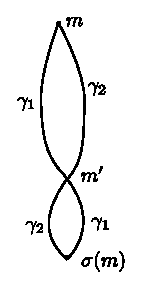
\includegraphics{figures/chap8-fig2.eps}
\end{figure}

\noindent
But \pageoriginale this contradicts (\ref{chap8:8.9.1}).
\end{proof}

\subsection{}\label{chap8:8.9.3}

\begin{coro*}
One has: $\text{ar}(M,g)\geq 4\pi$ and equality occurs if and only if
$A(M,g)=\{1\}$. 
\end{coro*}

\begin{proof}
By (\ref{chap8:8.9.2}), $(M,g)$ is $NCB(\pi)$. Then the results follows
from (\ref{chap8:8.4.7}) and (\ref{chap8:8.6.9}).
\end{proof}

\subsection{}\label{chap8:8.9.4}

\begin{lemma*}
Any closed geodesic $\gamma_{1}$ in $(M,g)$ meets any geodesic
$\gamma$ of length $\pi$.
\end{lemma*}

\begin{proof}
Let us suppose that they do not meet and that $\gamma$ is a geodesic
from $m$ to $\sigma(m)$. Then since $M$ is homeomorphic to the sphere
and $\gamma_{1}$ is a simple closed curve (by Jordan curve theorem) it
divides the rest of $M$ into two connected components. Since $\gamma$
is connected it is in one connected component. Let $m'$ be a point in
the other. Then let $\gamma_{2}$ be a geodesic curve from $m$ to
$\sigma(m)$ passing through $m'$. Then $m'$ and $\sigma(m)$ are in two
different connected components of $M-\gamma_{1}$ and $\gamma_{2}$ from
$m'$ to $\sigma(m)$ joins them. Hence $\gamma_{2}$ from $m'$ to
$\sigma(m)$ meets $\gamma_{1}$ and similarly $\gamma_{2}$ from $m$ to
$m'$ does. Hence $\gamma_{2}$ meets $\gamma_{1}$ in at least two
points $m_{1}$ and $m_{2}$. Then we have a part of the geodesic curve
$\gamma_{2}$, of length less than $\pi$, joining $m_{1}$ and $m_{2}$;
and a part of the geodesic curve $\gamma_{1}$ with the same
property. But this contradicts the fact that
$\exp_{m_{1}}|B(m_{1},\pi)$ is injective. Hence the result.
\end{proof}

\subsection{}\label{chap8:8.9.5}

\begin{theorem*}(L.W.\@ Green)
Let $(N,h)$ be an r.m.\@ such that
\begin{itemize}
\item[\rm i)] $N$ is homeomorphic to $P^{2}(\mathbb{R})$,

\item[\rm ii)] $(N,h)$ is a $C_{n}$-manifold $\forall n\in N$ (the
  common length being $\pi$). Then $(N,h)$ is isometric to
  $(P^{2}(\mathbb{R}),\can.)$. 
\end{itemize}
\end{theorem*}

\begin{proof}
\begin{enumerate}
\renewcommand{\theenumi}{\alph{enumi}}
\renewcommand{\labelenumi}{(\theenumi)}
\item Let \pageoriginale $A$ be a closed geodesic of length $2\pi$
  chosen once for all. It is a sub manifold of $(M,g)$. Using the
  notation of (\ref{chap8:sec8}) and (\ref{chap8:8.8.10}) we have
\begin{equation*}
\Vol(E_{\pi},\oob{g})\leq 8\pi^{2}.\tag{8.9.6}\label{chap8:8.9.6}
\end{equation*}

\item Now we claim that
$$
E_{\pi}=U(M)-U(M)|A.
$$
Since, any two geodesics through a point $m$ meet only at $\sigma(m)$
by the definition of $E_{\pi}$ it follows that
$$
E_{\pi}\subset U(M)-U(M)|A.
$$
Now let $x\in U(M)-U(M)|A$, and let $\gamma$ be the curve:
$$
t\to \exp t.x,\quad t\in [-\pi,0].
$$
But (\ref{chap8:8.9.4}) it follows that $\exists\, t_{0}\in [-\pi,0]$
such that $\exp(t_{0}x)\in A$ and hence, if we set $y=\gamma'(t_{0})$
we have $y\in U(M)|A$. Clearly since $A$ is a geodesic we have
$$
G_{t}(U(A))=U(A)
$$
and hence $y\not\in U(A)$. Further $t_{0}\neq -\pi$. Hence $y\in W$
and
$$
G_{-t_{0}}(y)=x\in E_{\pi}.
$$

\item Now since $U(M)|A$ is of measure zero in $U(M)$ we have\break by
  \eqref{chap5:5.2.13}
$$
\Vol(E_{\pi},\oob{g})=\Vol(U(M),\oob{g})=2\pi\cdot\text{ar}(M,g).
$$
But this together with \eqref{chap8:8.9.6} gives
$$
\text{ar}(M,g)\leq 4\pi.
$$
But then by (\ref{chap8:8.9.3}) we have first
\begin{align*}
\text{ar}(M,g) &= 4\pi,\\
\text{and then}\qquad A(M,g)=\{1\}.
\end{align*}
Now \pageoriginale by (\ref{chap7:7.7.1}) it follows that $(M,g)$ is
isometric to $(\mathbb{S}^{2},\can)$ and, since the deck
transformation $\sigma$ is such that
$$
d(m,\sigma(m))=\pi,
$$

$\sigma$ is nothing but the antipodal map of $\mathbb{S}^{2}$ hence
$(N,h)$ is isometric to $(P^{2}(\mathbb{R}),\can)$.
\end{enumerate}
\end{proof}

\setcounter{subsection}{6}

\subsection{}\label{chap8:8.9.7}

\begin{remarks*}
\begin{enumerate}
\renewcommand{\labelenumi}{\theenumi)}
\item The theorem was proved by Green under a slightly different
  assumption, namely that $(M,g)$ is a complete two dimensional r.m.\@
  such that $j(x)=\pi$ for every $x$ in $U(M)$. In this form, the
  theorem was conjectured by Blaschke a long time ago.

\item In the proof of (\ref{chap8:8.9.5}) one can replace the use of
  (\ref{chap8:8.8.10}) by that of (\ref{chap8:8.12.9}).

\item The question is open for the $P^{d}(\mathbb{R})$'s, $d\geq 3$.
\end{enumerate}
\end{remarks*}

\section{Concerning $G$-spaces}\label{chap8:sec10}

In order to bring out the results that are special to riemannian
geometry and do not belong to distance geometry in general, H.Busemann
was led to introduce metric spaces having the following properties.
\begin{itemize}
\item[i)] Every closed bounded set is compact.

\item[ii)] Any two points can be joined by a geodesic.

\item[iii)] Geodesics can be prolonged locally.

\item[iv)] These prolongations are unique.
\end{itemize}

The results that follow are in \cite{7}; the precise definition of the
spaces is as follows.

\subsection{}\label{chap8:8.10.1}\pageoriginale
{\em A $G$- space} $M$ is a metric space $M$ whose distance map $d$
verifies the following conditions:
\begin{itemize}
\item[i)] every closed bounded set is compact;

\item[ii)] $\forall m$, $n\in M$, $\exists\, p$ such that
$$
p\neq m, p\neq n\text{ \ and \ } d(m,n)=d(m,p)+d(p,n);
$$

\item[iii)] $\forall a\in M\exists\, r_{a}>0$ such that $\forall m$,
  $n\in M$ with
\begin{gather*}
d(a,m)<r_{a}, d(a,n)<r_{a},\exists\, p\text{ \  with}\\
p\neq m, p\neq n\text{ \ and \ }d (m,p) = d(m,n)+d(n,p);
\end{gather*}

\item[iv)] if $m$, $n\in M$ and $p_{1}$, $p_{2}$ are such that
$$
d(m,p_{i})=d(m,n)+d(n,p_{i})(i=1,2),d(n,p_{1})=d(n,p_{2})
$$
then $p_{1}=p_{2}$.
\end{itemize}
Under the above conditions i) and ii) one can define a set analogous
to $\mathscr{T}(m,n)$ and the notion of geodesics. Then iii) gives
local prolongability and iv) uniqueness of such prolongations.

Whether a $G$-space is necessarily a topological manifold is an open
question in dimensions greater than two.

Now any complete r.m.\@ is indeed a $G$-space; for i) comes from
(\ref{chap7:7.4.3}); ii) follows from (\ref{chap7:7.4.8}), iii) comes from
the existence of nice balls and iv) from (\ref{chap7:7.3.6}).

The essential result of Busemann is that the theorem (\ref{chap7:7.5.5})
pertains to $G$-spaces theory, whereas the theorems (\ref{chap8:8.7.3}) and
(\ref{chap8:8.9.5}) pertain to riemannian geometry.

Concerning (\ref{chap7:7.5.5}) the first thing to do is to find a metric
definition equivalent to that of non positive curvature for a r.m.;
such a definition is suggested by (\ref{chap7:7.3.8}); in a $G$-space 
$M$ \pageoriginale and inside a ball $D(a,r_{a})=\{m\in
M|d(a,m)<r_{a}\}$ one proves the uniqueness of a geodesic between two
points, in particular of a midpoint $(n,n',\frac{1}{2}) \; \forall n$,
$n'\in D(a,r_{a})$, defined by
$$
d(n,(n,n',\frac{1}{2}))+d((n,n',\frac{1}{2}),n')=d(n,n').
$$
Then

\subsection{}\label{chap8:8.10.2}

\begin{defi*}
A $G$-space is said to have non positive curvature if \; $\forall a\in
M\exists\, \circ <s_{a}<r_{a}$ such that
$$
d((m,n,\frac{1}{2}),(m,n',\frac{1}{2}))\leq\frac{1}{2}d(n,n') \; \forall
n,n'\in D(a,s_{a}).
$$
Then Busemann proved the following theorems \cite{7} (38.2) and (39.1):
\end{defi*}

\subsection{}\label{chap8:8.10.3}

\begin{theorem*}
A simply connected $G$-space $M$ with non positive curvature is such
that one can take $r_{a}=\infty$ in (\ref{chap8:8.10.1}) iii) $\forall a\in
M$. In particular any two geodesics in $M$ meet in at most one point
and $M$ is homeomorphic to some $\mathbb{R}^{d}$.
\end{theorem*}

On the other hand the theorems of L.W.\@ Green and E.\@ Hopf are not
true for $G$-spaces, as shown by the following

\subsection{}\label{chap8:8.10.4}

\begin{theorem*}(\cite{7}, theorem (33.3))
There exists on $\mathbb{S}'\times \mathbb{S}$ a $G$-space structure
whose universal covering is not isomorphic to the canonical $G$-space
$\mathbb{R}^{2}$, such that any two geodesics meet at most at one point.
\end{theorem*}

Theorem (33.3) of \cite{7} gives far more: it characterizes completely
the systems of curves in $\mathbb{R}^{2}$ which are the set of
geodesics of the universal covering of a $G$-space structure on
$\mathbb{S}^{1}\times\mathbb{S}^{1}$; then it is easy to pick out such
a system which is not arguesian, although the canonical $G$-space
structure on $\mathbb{R}^{2}$ is arguesian.

\subsection{}\label{chap8:8.10.5}

\begin{theorem*}(Skornyakov: \cite{28}, see also   \cite{8})
Let\pageoriginale $\sum$ be any system of closed Jordan curves in
$P^{2}(\mathbb{R})$ such that any two distinct points in
$P^{2}(\mathbb{R})$ lie exactly on one curve of $\sum$. Then there
exists a $G$-space structure on $P^{2}(\mathbb{R})$ whose set of
geodesics is $\sum$.
\end{theorem*}

\section{Conformal representation}\label{chap8:sec11}

If $(M,g)$ is an oriented surface we can define a map
$$
J:T(M)\to T(M)
$$
by extending linearly the map
$$
x\to \ub{x}
$$
appearing in the beginning of the proof of (\ref{chap8:8.6.2}). It
follows directly from the definition that the map $J$ has the
following properties:
\begin{itemize}
\item[(i)] $J^{2}=-\id_{T(M)}$

\item[(ii)] $g\circ J=g$

i.e. $g(J\circ X,J\circ Y)=g(x,Y)$, $\forall X$, $Y\in \mathscr{C}(M)$

\item[(iii)] If $f:M\to M$ is an isometry, then
\begin{align*}
& f^{T}\circ J=J\circ f^{T} \text{ \ if $f$ preserves orientation,}\\
& f^{T}\circ J=-J\circ f^{T}\text{ \ if $f$ reverses orientation.}
\end{align*}

\item[(iv)] If $h$ is any other r.s.\@ on $M$ such that $h\circ J=h$
  then there exists a $\varphi$ in $F(M)$ such that $h=\varphi\cdot
  g$. Now suppose that on the tangent bundle $T(M)$ of an even
  dimensional manifold $M$ a map $J$
$$
J:T(M)\to T(M)
$$
satisfying \pageoriginale the equation
$$
J^{2}=-\id_{T(M)}
$$
is given. Then in order that there exists on $M$ a complex analytic
structure for which $J$ coincides with the multiplication by $i$ it is
necessary and sufficient that the map defined by
\begin{gather*}
[X,Y]-J\circ [J\circ X,J\circ Y]+J\circ[J\circ X,Y]+[J\circ X,J\circ
  Y]=0\\
\forall X, Y\in\mathscr{C}(M)
\end{gather*}
be the zero map: see \cite{23}.
\end{itemize}

In the case of our $(M,g)$, because of the bilinearity of the
expression above, we can assume that $J\circ X=Y$ in the expression
above; then it is zero. Hence it follows that every two dimensional
oriented r.m.\@ admits a complex analytic structure the associated $J$
of which satisfies ii).

This construction, applied to $(\mathbb{S}^{2},\can)$ leads to the
Riemann sphere.

\subsection{}\label{chap8:8.11.1}

\begin{remark*}
In out two dimensional case for the existence, we do not actually need
the deep theorem of \cite{23}. What we need is ``the existence of
isothermal coordinates'' which is easier: see \cite{10}. {\em Now for
  the rest of this article, let} $\widetilde{h}_{0}$ denote the
canonical r.s.\@ on $\mathbb{S}^{2}$, and $h_{0}$ the canonical r.s.\@
on a flat torus (see (\ref{chap3:3.2.2})) or that on $P^{2}(\mathbb{R})$. It
is clear that a flat torus admits a canonical complex structure,
coming down from that of $\mathbb{R}^{2}$, and we denote the
associated multiplication by $\sqrt{-1}$ on its tangent bundle by
$J_{0}$; we denote also by $J_{0}$ the multiplication by $\sqrt{-1}$
on the tangent bundle of the Riemann sphere
$(\mathbb{S}^{2},\widetilde{h}_{0})$. Then the conformal
representation theorem \pageoriginale for Riemann surface gives, in
particular the 
\end{remark*}

\subsection{}\label{chap8:8.11.2}

\begin{theorem*}
Let $M$ be a one dimensional complex manifold. Then
\begin{enumerate}
\renewcommand{\theenumi}{\roman{enumi}}
\renewcommand{\labelenumi}{\rm\theenumi)}
\item if $M$ is homeomorphic to $\mathbb{S}^{1}\times\mathbb{S}^{1}$
  there exists a flat torus $(N,h_{0})$ and a diffeomorphism
$$
\lambda:N\to M
$$
such that
$$
\lambda^{T}\circ J_{0}=J\circ \lambda^{T}
$$

\item if $M$ is homeomorphic $\mathbb{S}^{2}$ there exists a
  diffeomorphism $\lambda:\mathbb{S}^{2}\to M$ such that
$$
\lambda^{T}\circ J_{0}=J\circ \lambda^{T}
$$
(the condition $\lambda^{T}\circ J_{0}=J\circ \lambda^{T}$ simply
means indeed that $\lambda$ is holomorphic).
\end{enumerate}

Now suppose that we take the complex analytic structure associated to
the r.s.\@ $g$ on $(M,g)$. Then on the flat torus $(N,h_{0})$ or on
$(\mathbb{S}^{2},\can)$
$$ 
\lambda^{\ast}(g)\circ J_{0}=g\circ \lambda^{T}\circ J_{0}=g\circ
J\circ \lambda^{T}=g\circ \lambda^{T}=\lambda^{\ast}(g)
$$
which together with (iv) gives the
\end{theorem*}

\subsection{}\label{chap8:8.11.3}

\begin{prop*}
Let $(N,g)$ be an r.m. Then
\begin{enumerate}
\renewcommand{\labelenumi}{\rm(\theenumi)}
\item if $M$ is homeomorphic to $\mathbb{S}^{1}\times \mathbb{S}^{1}$
  then there exists a flat torus $(N,h_{0})$ and a diffeomorphism
  $\lambda:N\to M$ and a $\varphi\in F(N)$ such that
  $\lambda^{\ast}(g)=\varphi\cdot h_{0}$.

\item if $M$ is homeomorphic to $\mathbb{S}^{2}$, then there exists a
  diffeomorphism $\lambda:\mathbb{S}^{2}\to M$ and a $\varphi\in
  F(\mathbb{S}^{2})$ such that $\lambda^{\ast}(g)=\varphi\cdot
  \widetilde{h}_{0}$.
\end{enumerate}
\end{prop*}


\subsection{}\label{chap8:8.11.4}

\begin{coro*}
Let\pageoriginale $(M,g)$ be an r.m.\@ that is homeomorphic to
$P^{2}(\mathbb{R})$. Then there exists a diffeomorphism
$$
\lambda:P^{2}(\mathbb{R})\to M\text{ \ and a \ }\varphi\in
F(P^{2}(\mathbb{R}))\text{ \ such that}
$$
$\lambda^{\ast}(g)=\varphi\cdot h_{0}$.
\end{coro*}

\begin{proof}
Let $(\widetilde{M},\widetilde{g})$ be the universal riemannian
covering of $(M,g)$
\[
\xymatrix@R=.5cm{
(\widetilde{M},\widetilde{g})\ar[dd]^{p} &\\
 & (p^{\ast}(g)=g)\\
(M,g)
}
\]
Then $\widetilde{M}$ is homeomorphic to $\mathbb{S}^{2}$ and for the
$J$ associated to $g$ and by (\ref{chap8:8.2.3}), there exists a
diffeomorphism $\mu:\mathbb{S}^{2}\to M$ such that
$$
\mu^{T}\circ J_{0}=J\circ \mu^{T}
$$
Let us denote the non trivial deck transformation of $\widetilde{M}$
by $\widetilde{\sigma}$ and set
$$
\widehat{\sigma}=\mu^{-1}\circ\widetilde{\sigma}\circ\mu
$$
The deck transformation $\widetilde{\sigma}$ is an isometry (see in
(\ref{chap7:7.6.5})) reversing the orientation and hence by (iii) we have
$$
\widetilde{\sigma}^{T}\circ J=-J\circ \widetilde{\sigma}^{T}
$$
which gives
$$
\widehat{\sigma}^{T}\circ J_{0}=-J\circ\widehat{\sigma}^{T}
$$
Hence $\widehat{\sigma}$ is an automorphism of $\mathbb{S}^{2}$ which
reverses the sign of $J$, i.e.\@ an antiholomorphic map, and further
$\widehat{\sigma}$ is an involution without fixed points (since
$\widetilde{\sigma}$ is). All antiholomorphic maps of the Riemann
sphere being of the type
$$
z\to \dfrac{a\overline{z}+b}{c\overline{z}+d}
$$
one \pageoriginale deduces that there exists a holomorphic map
$\theta:\mathbb{S}^{2}\to \mathbb{S}^{2}$ such that
$\widehat{\sigma}=\theta\circ \sigma\circ \theta^{-1}$ where
$\sigma= -\id|\mathbb{R}^{3}|\mathbb{S}^{2}$ is the antipodal map on
$\mathbb{S}^{2}$. Now if we set $\widetilde{\lambda}=\mu\circ\theta$
then $\widetilde{\lambda}$ is a diffeomorphism between
$\mathbb{S}^{2}$ and $M$ and we have
$$
\widetilde{\lambda}^{-1}\circ\widetilde{\sigma}\circ\widetilde{\lambda}=\sigma
$$
and hence we have a map $\lambda$ defined by the following commutative
diagram
\[
\xymatrix@C=1.8cm{
(\widetilde{M},\widetilde{g})\ar[d]_{p} &
  (\mathbb{S}^{2},\widetilde{h}_{0})\ar[d]^{p}\ar[l]_{\widetilde{\lambda}}\\
(M,g) & (P^{2}(\mathbb{R}),h_{0})\ar[l]_{\lambda}
}
\]
Since $\widetilde{\lambda}$ is holomorphic by (iv) there exists a
$\psi$ in $F(\mathbb{S}^{2})$ such that
$$
(\widetilde{\lambda})^{\ast}(\widetilde{g})=\psi\widetilde{h}_{0}.
$$
We have
$$
(\widetilde{\lambda})^{\ast}(\widetilde{g})=\widetilde{\lambda}^{\ast}(p^{\ast}(g))=p^{\ast}(\lambda^{\ast})(g) 
$$
and hence
$$
p^{\ast}((\lambda^{\ast}(g))=\psi p^{\ast}(h_{0})
$$
which implies, since $p^{T}$ is of maximal rank, that there exists a
$\varphi$ in $F(P^{2}(\mathbb{R}))$ such that
$$
\psi=\varphi\cdot p\quad\text{and}\quad \lambda^{\ast}(g)=\varphi\cdot
h_{0}
$$
Hence the result.
\end{proof}

\section{The theorems of Loewner and Pu}\label{chap8:sec12}

In this article we consider a given manifold $M$ of dimension two and
various r.s.\@ on it.

{\em We set}
$$
a(g)=\text{ar}(M,g)
$$
{\em and \pageoriginale in case $\overline{F}(M)$ is non trivial} (see
(\ref{chap7:sec6}))  
$$
c(g)=\inf\{\lg(\tau))|\tau\in\overline{F}(M)-\{0\}\}
$$
i.e.\@ $c(g)$ is the infimum of the lengths of all closed curves in
$(M,g)$ which are not homotopic to zero. The theorem of Loewner gives
a lower bound for $\dfrac{a(g)}{(c(g))^{2}}$ for any r.s.\@ on
$\mathbb{S}^{1}\times \mathbb{S}^{1}$ and that of $P_{u}$ in the case
of $P^{2}(\mathbb{R})$. Before giving them we compute
$a(g)/(c(g))^{2}$ in the standard cases.
\begin{enumerate}
\renewcommand{\theenumi}{\Alph{enumi}}
\renewcommand{\labelenumi}{\theenumi)}
\item Let us take $P^{2}(\mathbb{R})$ and denote its canonical r.s.\@
  by $h_{0}$. By \eqref{chap6:6.7.6} $a(h_{0})=2\pi$. To compute $c(h_{0})$
  we look at the universal riemannian covering:
$$
(\mathbb{S}^{2},\can)\quad (P^{2}(\mathbb{R}),h_{0}).
$$
For every $\tau$ in $\overline{F}(P^{2}(\mathbb{R}))-\{0\}$ the lift
$\overline{\tau}$ of $\tau$ through $m$ ends in
$\sigma(m)(\sigma=-\id_{\mathbb{R}^{3}}|\mathbb{S}^{2})$ so that
$\lg(\widetilde{\tau})\geq \pi$ and equality occurs if
$\widetilde{\tau}$ is a geodesic. Hence we have
\begin{equation*}
\frac{a(h_{0})}{c^{2}(h_{0}))^{2}}=\frac{2}{\pi}.\tag{8.12.1}\label{chap8:8.12.1}
\end{equation*}

\item Now let us take a flat torus
  $(T,h_{0})=(\mathbb{R}^{2}/G,\epsilon/G)$.

Let us denote the metric on $(\mathbb{R}^{d},\epsilon)$ by $\rho$. Now
let $\{s,t\}$ be a system of generators of $G$ such that
$$
\rho(0,s(0))=\inf\{\rho(0,k(0))|k\neq 0, k\in G\}.
$$
We set $a=s(0)$ and $b=t(0)$. To compute $c(h_{0})$ we look at the
universal riemannian covering:
$$
(\mathbb{R}^{2},\epsilon)\to (T,h_{0}).
$$
By our selection of $s$ it follows that the lift of any closed curve
$\tau$ is such that
$$
\lg(\tau)=\lg(\widetilde{\tau})\geq \rho(0,a),
$$
and \pageoriginale equality is attained. Further we have
$$
\rho(0,a)\leq \rho(0,b),\quad\text{and}\quad \rho(0,a)\leq \rho(a,b)
$$
because $s-t\in G$, we have
$$
c(h_{0})\leq \frac{1}{3}\quad\text{(perimeter of $0ab$)}.
$$
On the other hand we have by {(\ref{chap3:3.5.7})}
$$
a(h_{0})=\det(\overline{0a},\overline{0b})=2\quad\text{(area of
  $0ab$)}.
$$
But the well known isoperimetric inequality for triangles gives that
\begin{equation*}
\text{(area of $0ab$)}\leq \frac{\sqrt{3}}{36}\quad\text{(perimeter of
  $0ab$)$^{2}$}\tag{8.12.2}\label{chap8:8.12.2} 
\end{equation*}
where equality occurs if and only if $0ab$ is equilateral.
\end{enumerate}

\setcounter{subsection}{2}

\subsection{}\label{chap8:8.12.3}

\begin{defi*}
A flat torus in $\mathbb{R}^{2}$ is said to be equilateral if there
exists a similitude of $\mathbb{R}^{2}$ transforming it into the torus
got by the group $G$ generated by
$$
s:0\to s=(0,1)\quad\text{and}\quad t:0\to
t=\left(\frac{1}{2},\frac{3}{2}\right). 
$$
Then by \eqref{chap8:8.12.2} we have
\end{defi*}

\subsection{}\label{chap8:8.12.4}

\begin{lemma*}
For a flat torus
$$
a(h_{0})/c^{2}(h_{0})\geq \dfrac{\sqrt{3}}{2}
$$
where equality occurs if and only if the torus is equilateral.
\end{lemma*}

\begin{enumerate}
\renewcommand{\theenumi}{\Alph{enumi}}
\renewcommand{\labelenumi}{\theenumi)}
\setcounter{enumi}{2}
\item The underlying idea of the proofs of the theorems of Loewner and
  Pu is as follows: first using 11 we get an isometry between $(M,g)$
  and an r.s.\@ of the type $\varphi\cdot h_{0}$ on the standard
  manifold. Then we use the transitive group of isometries these
  standard manifolds possess to average the function $\varphi$ in such
  a way $a(h)$ decreases and $c(h)$ increases. First \pageoriginale we prove two
  lemmas, relative to the following situation: $(N,\epsilon)$ is a
  compact surface and $\mathscr{C}$ a compact Lie group operating
  transitively, by isometries, on $(N,\epsilon)$; denote by $\tau$ any
  volume form on $\mathscr{C}$ such that
$$
\Vol(\mathscr{C})=\int\limits_{\mathscr{C}}\tau=1.
$$
We suppose given on $N$ an everywhere strictly positive function and
we consider the average $\widehat{\varphi}$, by $\mathscr{C}$, of its
square root, i.e.\@ we set
$$
\widehat{\varphi}=\left(\int\limits_{t\in\mathscr{C}}(\varphi\circ
t)^{\frac{1}{2}}\cdot\tau\right)^{2}. 
$$
In this context we have the following two lemmas.
\end{enumerate}

\subsection{}\label{chap8:8.12.5}

\begin{lemma*}
$a(\widehat{\varphi}\cdot\epsilon)\leq a(\varphi\cdot\epsilon)$ and
  the equality holds if and only if the function $\varphi$ is constant
  on $N$.
\end{lemma*}

\begin{proof}
Let $\sigma_{\varphi\epsilon}$ be the volume element of the r.m.\@
$(N,\varphi\cdot\epsilon)$; by (\ref{chap3:3.5.4}),
$\sigma_{\varphi\epsilon}=\varphi\sigma_{\epsilon}$ so that
$$
a(\widehat{\varphi}\cdot\epsilon)=\int\limits_{N}
\sigma_{\widehat{\varphi}\epsilon}=\int\limits_{N}
\widehat{\varphi}\sigma_{\epsilon}=\int\limits_{N}\int\limits_{\mathscr{C}}(\varphi\circ
t)^{\frac{1}{2}}\cdot\tau)^{2}\sigma_{\epsilon}; 
$$
by Schwarz' inequality
$$
\left(\int\limits_{\mathscr{C}}(\varphi\circ
t)^{\frac{1}{2}}\cdot\tau\right)^{2}\leq
\int\limits_{\mathscr{C}}(\varphi\circ t)\cdot
\tau\int\limits_{\mathscr{C}}\tau
=\int\limits_{\mathscr{C}}(\varphi\circ t)\cdot \tau
$$
and
$$
a(\widehat{\varphi}\cdot\epsilon)\leq
\int\limits_{N\times\mathscr{C}}(\varphi\circ
t)(\tau\times\sigma_{\epsilon})=\int\limits_{t\in\mathscr{C}}\int\limits_{N}(\varphi\circ
t)\cdot \sigma_{\epsilon})\cdot\tau.
$$
But the fact that $t$ is an isometry implies that
$t^{\ast}\sigma_{\epsilon}=\sigma_{\epsilon}$ and hence
\begin{align*}
\int\limits_{N}(\varphi\circ t)\cdot
\sigma_{\epsilon}=\int\limits_{N}t^{\ast}\varphi\cdot
t^{\ast}\sigma_{\epsilon}
&=\int\limits_{N}t^{\ast}(\varphi\cdot\sigma_{\epsilon})=\int\limits_{N}\varphi
\sigma_{\epsilon}\quad\text{(by (\ref{chap0:0.3.15}))}\\
&=a(\varphi\cdot \epsilon);
\end{align*}
Consequently\pageoriginale
$$
a(\widehat{\varphi}\cdot\epsilon)\leq \int\limits_{t\in
  \mathscr{C}}a(\varphi\cdot \epsilon)\cdot\tau =a(\varphi\cdot
\epsilon)\cdot\Vol(\mathscr{C})=a(\varphi\cdot \epsilon). 
$$
Equality occurs if and only if it occurs in Schwarz' inequality, ie.\@
if and only if the function $t\to \varphi\circ t$ on $\mathscr{C}$ is
constant, which implies that $\varphi$ itself is constant because
$\mathscr{C}$ acts transitively on $N$.
\end{proof}

\subsection{}\label{chap8:8.12.6}

\begin{lemma*}
$c(\widehat{\varphi}\cdot\epsilon)\geq c(\varphi\cdot\epsilon)$.
\end{lemma*}

\begin{proof}
Let $\gamma$ be any curve in $N$; we suppose it given in the form
$\gamma:[0,1]\to N$. Then
\begin{align*}
\lg(\gamma,\widehat{\varphi}\cdot\epsilon) = 
&\int\limits^{1}_{0}((\widehat{\varphi}\cdot\epsilon)(\gamma',\gamma'))^{\frac{1}{2}}\cdot
\dt=\int\limits^{1}_{0}\widehat{\varphi}^{\frac{1}{2}}(\epsilon(\gamma'\cdot\gamma')^{\frac{1}{2}}\dt=\\
&= \int\limits^{1}_{0}\left(\int\limits_{t\in\mathscr{C}}(\varphi\circ
t)^{\frac{1}{2}}\cdot\tau\right)(\epsilon(\gamma',\gamma'))^{\frac{1}{2}}\cdot
\dt=\\
&=\int\limits_{[0,1]\times\mathscr{C}}(\varphi\circ
t)^{\frac{1}{2}}(\epsilon(\gamma',\gamma'))^{\frac{1}{2}}\cdot\tau\times
\dt=\\
&=\int\limits_{\mathscr{C}}\left(\int\limits^{1}_{0}(((\varphi\circ
t)\cdot \epsilon)(\gamma',\gamma'))^{\frac{1}{2}}\cdot \dt\right)\tau
\end{align*}
But since $t$ is an isometry
\begin{align*}
((\varphi\circ t)\epsilon)(\gamma',\gamma') &= (t^{\ast}\varphi\cdot
  t^{\ast}\epsilon)(\gamma',\gamma')=t^{\ast}(\varphi\cdot
  \epsilon)(\gamma',\gamma')=\ldots\\
\ldots &= (\varphi\cdot\epsilon)(t^{T}\circ
\gamma',t^{T}\circ\gamma')=(\varphi\cdot\epsilon)(t\circ
\gamma)',(t\circ \gamma)').
\end{align*}
Now
$$
\int\limits^{1}_{0}((\varphi\cdot \epsilon)(t\circ
\gamma)',(t\circ\gamma))^{\frac{1}{2}}\cdot \dt=\lg(t\circ
\gamma,\varphi\cdot \epsilon)
$$
so we get
$$
\lg(\gamma,\widehat{\varphi}\cdot\epsilon)=\int\limits_{t\in\mathscr{C}}\lg(t\circ\gamma,\varphi\cdot\epsilon)\cdot \tau.
$$
Suppose \pageoriginale now that $\tau$ is closed and non homotopic to
zero in $N$; then the same holds for the curves $t\circ \gamma$,
because the $t$'s are diffeomorphisms; hence by the definition of
$c(\varphi\cdot \epsilon)$, 
$$
\lg(\gamma,\widehat{\varphi}\cdot\epsilon)\geq
\int\limits_{\mathscr{C}}c(\varphi\cdot\epsilon)\cdot\tau=c(\varphi\cdot\epsilon)\cdot\Vol(\mathscr{C})=c(\varphi\cdot\epsilon). 
$$
Now this holds for any such $\gamma$, so that, by the definition of
$c(\widehat{\varphi}\cdot\epsilon)$, we get
$$
c(\widehat{\varphi}\cdot\epsilon)\geq c(\varphi\cdot\epsilon).
$$
\end{proof}


\subsection{}\label{chap8:8.12.7}

\begin{prop*}
With the hypothesis of the lemmas, we have
$$
\frac{a(\varphi\cdot\epsilon)}{(c(\varphi\cdot\epsilon))^{2}}\geq
\frac{a(\epsilon)}{(c(\epsilon))^{2}} 
$$
and equality holds if and only if $\varphi$ is constant.
\end{prop*}

\begin{proof}
We have only to remark that the transitivity of $\mathscr{C}$ implies
the average $\widehat{\varphi}$ is constant on $N$; let $k$ be that
constant value, then $a(\widehat{\varphi}\cdot\epsilon)=k^{2}\cdot
a(\epsilon)$ and $c(\widehat{\varphi}\cdot\epsilon)=k\cdot
c(\epsilon)$; hence the two lemmas yield
$$
\frac{a(\varphi\cdot\epsilon)}{(c(\varphi\cdot\epsilon))^{2}}\geq
\frac{k^{2}\cdot a(\epsilon)}{k^{2}\cdot
  (c(\epsilon))^{2}}=\frac{a(\epsilon)}{(c(\epsilon))^{2}} 
$$
\end{proof}

\subsection{}\label{chap8:8.12.8}

\begin{coro*}(Loewner, unpublished)
Let $(M,g)$ be such that $M$ is homeomorphic to
$\mathbb{S}^{1}\times\mathbb{S}^{1}$. Then
$$
\frac{a(g)}{(c(g))^{2}}\geq\frac{\sqrt{3}}{2}
$$
where equality holds if and only if $(M,g)$ is isometric to an
equilateral flat torus.
\end{coro*}

\begin{proof}
By \eqref{chap8:8.2.3} there exists a flat torus $(N,h)$, a diffeomorphism
$f$ from $N$ to $M$ and $\varphi\in F(N)$ such that
$$
f^{\ast}(g)=\varphi\cdot h.
$$
So \pageoriginale that $(M,g)$ and $(N,\varphi,h)$ are isometric under
$f$ and in particular
$$
a(g)=a(\varphi\cdot h),\quad c(g)=c(\varphi\cdot h).
$$
Now the corollary follows from (\ref{chap8:8.12.7}) combined with
(\ref{chap8:8.12.4}).
\end{proof}

\subsection{}\label{chap8:8.12.9}

\begin{coro*}(Pu: \cite{25})
Let $(M,g)$ be such that $M$ is homeomorphic to
$P^{2}(\mathbb{R})$. Then
$$
\frac{a(g)}{(c(g))^{2}}\geq\frac{2}{\pi}
$$
where equality holds if and only if there is $k>0$ such that $(M,g)$
is isometric to $(P^{2}(\mathbb{R}),k.\can)$.
\end{coro*}

\begin{proof}
This time we get the transitive group $\mathscr{C}$ of isometries of
$(P^{2}(\mathbb{R})\cdot\can)$ by writing $P^{2}(\mathbb{R})$ as the
homogeneous space
$$
P^{2}(\mathbb{R})=S0(3)/0(2).
$$
\end{proof}

\subsection{}\label{chap8:8.12.10}

\begin{remarks*}
\begin{enumerate}
\renewcommand{\theenumi}{\Alph{enumi}}
\renewcommand{\labelenumi}{\theenumi.}
\item The result (\ref{chap8:8.12.8}) has been generalized by Blatter in
  \cite{5}, to compact orientable manifolds of genus $\gamma\geq 2$;
  precisely: for any integer $\gamma\geq 2$ there exists a real number
  $n_{\gamma}$ such that
$$
\frac{a(g)}{(c(g))^{2}}\geq n_{\gamma}
$$
for any surface $(M,g)$ where $M$ is compact, orientable, of genus
$\gamma$. The proof is definitely deeper than the one above. {\em But
  here the equality} is never attained. We sketch here the proof
(based on an idea of N. Kuiper): suppose $(M,g)$ is such that the
equality is attained and {\em call $m$-curve} in $(M,g)$ a curve of
length equal to $c(g)$ (they are closed geodesics); then first: given
any point $m\in M$ and any neighbourhood $V$ of \pageoriginale $m$
there exists an $m$-curve which meets $V$ (in fact, if not, change
slightly the r.s.\@ inside $V$ in order to have a smaller $a(g)$; this
change would not affect $c(g)$ and so it is impossible). By continuity
one shows now that $\forall m\in M$ there exists a one-parameter
family $f$ of $m$-curves such that $f(0,0)=m$. Looking at the
corresponding Jacobi fields, such a Jacobi field either never vanishes
or vanishes at least at two points (thanks to the fact that $M$ is
oriented); but it cannot vanish at two points for (\ref{chap8:8.2.9})
would imply that the geodesic is not an $m$-curve. Finally following
such a family by continuity one would get a vector field on $M$, which
is never zero, contradicting the fact that the genus of $M$ is greater
than one.

\item The theorems of Loewner and Pu are answers to particular cases
  of the following general question: given a compact differentiable
  manifold $M$ and some homology or homotopy class or set of classes
  $\delta$, and an r.s.\@ $g$ on $M$, set
$$
a(g)=\Vol(M,g)\quad\text{and}\quad
c(g)=\inf\{\Vol(N,g|N)|N\in\delta\}.
$$
Then: does one have an inequality $a(g)\geq k\cdot (c(g))^{n}$, valid
for any $g$; if so, what are the cases of equality? (the integer $n$
is defined so that the quotient $\dfrac{a(g)}{(c(g))^{n}}$ be
homogeneous of degrees zero).
\end{enumerate}
\end{remarks*}

The good candidates for generalizing the Pu theorem are the
S.C.-manifolds (excepting the spheres), when one takes for $\delta$
the class of a projective subspace. Except in the case of
$P^{2}(\mathbb{R})$ the \pageoriginale question is completely
open. However, the answer cannot be so simple; in fact, for the
complex projective space either $k$ has not the value of the canonical
r.s.\@ or the equality can be attained for an r.s.\@ non isometric to
the canonical one. The proof of this fact consists simply in deforming
the canonical k\"ahlerian r.s.\@ by adding to it $\sqrt{-1}\cdot
d'd''f$ (where $f$ is a real function); Stokes formula (\ref{chap0:0.3.13})
and an inequality of Wirtinger show easily that both $a(g)$ and $c(g)$
are unchanged.



\begin{thebibliography}{99}
\bibitem{1} W.\@ AMBROSE {\em Parallel Translation of Riemannian
  curvature}, Ann.\@ of Math., 64(1956) pp.337-363.

\bibitem{2} W.\@ AMBROSE, R.S.\@ PALAIS AND I.M.\@ SINGER {\em
  Sprays}, Acad. Brasilenia de Ciencas, 32 (1960), pp.\@ 163-178.

\bibitem{3} A.\@ AVEZ {\em Valeur moyenne du scalaire de courbure sur
  une vari\'et\'e compacte}, C.R.A.S.\@ Paris, 256(1963),
  pp.5271-5273.

\bibitem{4} W.\@ BLASCHKE {\em Differential Geometrie}, Springer.

\bibitem{5} C.\@ BLATTER {\em Uber Extremall\"angen auf geschlossenen
  Fl\"achen}, Comm. Math. Helv., 35(1961), pp.153-168.

\bibitem{6} R.\@ BOTT {\em On manifolds all of whose geodesics are
  closed}, Ann.\@ of Math., 60(1954), pp.375-382. 

\bibitem{7} H.\@ BUSEMANN {\em The Geometry of Geodesics}, Academic Press.

\bibitem{8} H.\@ BUSEMANN {\em Metrizations of Projective Spaces},
  Proc.\@ Am.\@ Math.\@ Soc., 81(1957), pp.387-390.

\bibitem{9} S.S.\@ CHERN {\em Topics in Differential Geometry},
  Inst.\@ for Adv.\@ Study. 

\bibitem{10} S.S.\@ CHERN {\em On isothermic coordinates}, Comm.\@
  Math.\@ Helv., 28(1954), pp.301-309.

\bibitem{11} A.I.\@ FET {\em Variational Problems on Closed
  Manifolds}, Am.\@ Math.\@ Soc.\@ Translations, No.\@ 90.

\bibitem{12} R.\@ GODEMENT {\em Th\'eorie des faisceaux}, Hermann.

\bibitem{13} L.W.\@ GREEN {\em Auf Wiedersehenfl\"ache}, Ann.\@ of
  Math., 78(1963), pp.289-299. 

\bibitem{14} S.\@ HELGASON {\em Differential Geometry and Symmetric
  Spaces}, Academic Press.

\bibitem{15} E.\@ HOPF {\em Closed surfaces without conjugate points},
  Prof.\@ Nat.\@ Acad.\@ Sc.\@ U.S.A., 34(1948), pp.47-51.

\bibitem{16} W.\@ KLINGENBERG {\em Riemannsche Geometrie im Grossen},
  Math.\@ Inst.\@ Univ.\@ Bonn.

\bibitem{17} S.\@ KOBAYASHI AND K.\@ NOMIZU {\em Differential
  Geometry}, Interscience Publishers.

\bibitem{18} J.L.\@ KOSZUL {\em Lectures on Fiber Bundles and
  Differential Geometry}, Tata Institute.

\bibitem{19} S.\@ LANG {\em Introduction to Differentiable Manifolds},
  Interscience Publishers.

\bibitem{20} A.\@ LICHNEROWICZ {\em Spineurs harmoniques}, C.R.A.S.\@
  Paris, 257(1963), pp.7-9.

\bibitem{21} J.\@ MILNOR {\em Morse Theory}, Princeton Univ.

\bibitem{22} S.B.\@ MYERS {\em Riemannian Manifolds with Positive Mean
  Curvature}, Duke Math.\@ Journ., 8(1941), pp.401-404.

\bibitem{23} A.\@ NEWLANDER AND L.\@ NIRENBERG {\em Complex Analytic
  Coordinates in Almost-Complex Manifolds}, Ann.\@ Math.,
  65(1957). pp.391-404.

\bibitem{24}

\bibitem{25} P.M.\@ PU {\em Some Inequalities in Certain non
  Orientable Manifolds}, Pacific Journ., 11(1952), pp.55-71.

\bibitem{26} G.\@ de RHAM {\em Vari\'et\'es differentiables}, Hermann.

\bibitem{27} L.A.\@ SANTALO {\em Integral Geometry in General Spaces},
  Proc.\@ International Congress of Math., 1950, pp.483-489.

\bibitem{28} L.A.\@ SKORMYAKOV {\em Metrization of the Projective
  Plane in connection with a Given System of Curves} (Russian),
  Izvest.\@ Akad.\@ Nauk S.S.S.R., ser.\@ Math., 19(1955) pp.471-482.

\bibitem{29} J.L.\@ SYNGE {\em On the Connectivity of Spaces of
  Positive Curvature}, Quarterly J.\@ of Math., 7(1936), pp.316-320.

\bibitem{30} ZOLL {\em Uber Fl\"achen mit Scharen geshclossener
  geod\"atischer Linian} (mit 3 Figuren in Text), Math.\@ Ann.,
  57(1903), pp.108-

\bibitem{31} J.\@ LELONG-FERRAND {\em G\'eom\'etrie diff\'erentielle},
  Masson. 

\bibitem{32} H.\@ SAMELSON {\em On Manifolds with Many Closed
  Geodesics}, Portugalise Mathematicae, 32(1963), pp.193-196.

\bibitem{33} R.\@ BISHOP AND R.\@ CRITTENDEN {\em Geometry of
  Manifolds}, Academic Press.

\bibitem{34} J.\@ NASH {\em The Imbedding Problem for Riemannian
  Manifolds}, Ann.\@ of Math., 63(1956), pp.20-63

\bibitem{35} S.\@ STERNBERG {\em Lectures on Differential Geometry},
  Prentice-Hall. 

\bibitem{36} J.\@ DIEUDONNE {\em Foundations of Modern Analysis,}
  Academic Press.

\bibitem{37} H.\@ FREUDENTHAL {\em Oktaven, Ausnahmegruppen und
  oktavengeometrie}, Math.\@ Inst.\@ Univ.\@ Utrecht.

\bibitem{38} E.\@ CARTAN {\em Sur certaines formes
  riemanniennes}\ldots (Ann.\@ Ec.\@ Norm.\@ sup., 44(1927), pp.345-467).
\end{thebibliography}

